% !TEX root =  free221.tex

\chapter{Limits and Continuous Functions}
While it is easy to define precisely in a few words what a square root
is ($\sqrt{a}$ is the positive number whose square is $a$) the
definition of the limit of a function is more complicated.  In this
chapter we will take three approaches to defining the limit.
The first definition (\S\ref{sec:informal-limit-def}) appeals to
intuition and puts in words how most people think about limits.
Unfortunately this definition contains language that is ambiguous and
the more you think about it the more you realize that it actually
doesn't mean anything.  It is also not clear enough to answer all questions that
come up about limits.

Most of the calculus you'll see in this semester was essentially invented
in the 17th century, but the absence of a good definition of what
derivatives and limits are led to centuries of confused arguments between
experts.  These more or less ended when a precise definition was developed
in the late 19th century, 200 years after calculus was born!  In
\S\ref{sec:formal-limit-def} you'll see this precise definition.  It runs
over several terse lines, and unfortunately most people don't find it very
enlightening when they first see it.
The third approach we will take is the \emph{axiomatic approach}:
instead of worrying about the details of what a limit is, we use our
intuition and in \S\ref{sec:limitProperties} we write down a number of
properties that we believe the limit should have.  After that we try
to base all our reasoning on those properties.

\section{Informal definition of limits} 
\label{sec:informal-limit-def}

\subsection{Definition of limit (1st attempt)} 
\itshape\label{def:limit-first-attempt}
If $f$ is some function then
\[
\lim_{x\to a} f(x) = L
\]
is read ``the limit of $f(x)$ as $x$ approaches $a$ is $L$.''  It
means that if you choose values of $x$ that are close \emph{but not
  equal} to $a$, then $f(x)$ will be close to the value $L$; moreover,
$f(x)$ gets closer and closer to $L$ as $x$ gets closer and closer to
$a$.  \upshape\smallskip

The following alternative notation is sometimes used
\[
f(x)\to L \quad\text{ as } \quad x\to a;
\]
(read ``$f(x)$ approaches $L$ as $x$ approaches $a$'' or ``$f(x)$ goes to
$L$ as $x$ goes to $a$''.)

Note that in the definition we require $x$ to approach $a$ without
ever becoming equal to $a$.  It's important that $x$ never actually
equals $a$ because our main motivation for looking at limits was
the definition of the derivative.  In Chapter II, equation
\eqref{eq:derivative-defined-first-time} we defined the derivative of
a function as a limit in which some number $\Delta x$ goes to zero:
\[
f'(x) = \lim_{\Delta x\to0} \frac{f(x+\Delta x)-f(x)}{\Delta x}.
\]
The quantity whose limit we want to take here is not even defined when
$\Delta x=0$.  Therefore any definition of limit we come up with had
better not depend on what happens at $\Delta x=0$; likewise, the limit
$\lim_{x\to a}f(x)$ should not depend on what $f(x)$ does at $x=a$.
\subsection{Example} 
If $f(x) = x+3$ then
\[
\lim_{x\to 4} f(x) = 7,
\]
is ``true'', because if you substitute numbers $x$ close to $4$ in $f(x) = x+3$
the result will be close to $7$.
\subsection{A complaint} 
Our first definition relies heavily on the
phrase ``gets close to'' or ``gets closer and closer to''.  What does
this mean?  When $x$ gets closer and closer to $a$ without ever being
equal to $a$, how long does this take? (``are we there yet?'') How
close is close enough?  Is it enough for $x$ and $a$ to be the same in
five decimals?  Fifty decimals?  It is hard to answer these questions without
generating new ones.

If we want to deal with limits with some measure of confidence that what we are
doing isn't ultimately nonsense, then we will need a better definition of limit.
Before going into that, let's look at a practical approach to finding limits.
To compute $\lim_{x\to a} f(x)$ we need to let $x$ get closer and closer to $a$;
we don't really know how to do that, but we can certainly grab a calculator or a
computer and compute $f(x)$ for several values of $x$ that are somewhat close to
$a$ ($a$ to two decimals, $a$ to three decimals, etc.)  If the values of $f(x)$
then begin to look like some fixed number we could guess that that number is the
limit \footnote{This idea of making better and better approximations is actually
a common approach in modern science: if you have a complicated problem (such as
predicting tomorrow's weather, or the next three decades' climate) that you
cannot solve directly, one thing often tried is changing the problem a little
bit, and then making approximations with a computer.  This activity is called
\emph{Scientific Computation}, a very active branch of modern mathematics.}.  

Here are two examples where we try to find a limit by calculating
$f(x)$ for a few values of $x$:

\subsection{Example: substituting numbers to guess a limit} 
\label{ex:limit-by-sub-good}
What (if anything) is
\[
\lim_{x\to 2}\frac{x^2 -2x}{x^2-4}?
\]
Here $f(x) = (x^2 - 2x)/(x^2-4)$ and $a=2$.


We first try to substitute $x=2$, but this leads to
\[
f(2) = \frac{2^2 - 2\cdot2}{2^2-4} = \frac 00
\]
which does not exist.  Next we try to substitute values of $x$ close but
not equal to $2$.  Table \ref{tbl:finding-limits} suggests that $f(x)$
approaches $0.5$.


\begin{table}[ht]
  \centering
  \begin{tabular}{ll}
    \toprule
    \quad$x$ & \quad$f(x)$ \\
    \midrule
    3.000000 & 0.600000\\
    2.500000 & 0.555556\\
    2.100000 & 0.512195\\
    2.010000 & 0.501247\\
    2.001000 & 0.500125\\
    $\downarrow$& \hfil$\downarrow$\hfil\\
    2 & \hfil limit?\hfil\\
    \bottomrule
  \end{tabular}
  \qquad\qquad
  \begin{tabular}{ll}
    \toprule
    \quad$x$ & \quad$g(x)$ \\
    \midrule
    1.000000 & 1.009990\\
    0.500000 & 1.009980\\
    0.100000 & 1.009899\\
    0.010000 & 1.008991\\
    0.001000 & 1.000000\\
    $\downarrow$& \hfil$\downarrow$\hfil\\
    0& \hfil limit?\hfil\\
    \bottomrule
  \end{tabular}
  \smallskip
% !!! Issue: should this table split into 2 tables to fill in the missing data for limits from below? (and to separate f and g from each other)
  
  \caption{Finding limits by substituting values of $x$ ``close to $a$.''
    (Values of $f(x)$ and $g(x)$ rounded to six decimals.)}
  \label{tbl:finding-limits}
\end{table}  

\subsection{Example: substituting numbers can suggest the wrong answer} 
\label{ex:limit-by-sub-bad}
Suppose we had the function
\[
g(x) = \frac{101\,000x}{100\,000x+1}
\]
and we want to find the limit $\lim_{x\to0}g(x)$.

Then substitution of some ``small values of $x$'' could lead us to believe
that the limit is $1.000\ldots$.  But in fact, if we substitute sufficiently
small values, we will see that the limit is $0$ (zero)!
As you see from this example, there's more to evaluating limits
than just typing numbers into the computer and hitting return.  See
also problem \ref{ex:bad-calculator-bad}.
\section{Problems} 
\problemfont 
\begin{multicols}{2}
\problem Guess $\lim_{x\to 2} x^{10}$. 
Then try using the first definition of the limit to show that your
guess is right.
\problem Use a calculator to guess the value of 
\[
\lim_{x\to0} \bigl(1+x\bigr)^{1/x}.
\]

\problem Is the limit 
$\lim_{x\to0} (1+0.693x)^{1/x}$
an integer?  Give reasons for your answer, and compare with your
neighbor's answer.

\problem Simplicio computed $2^{-10} \approx 0.001$ which is very 
close to zero.  He therefore concludes that if $x$ is very close to
$2$, then $x^{-10}$ is very close to zero, so that, according to
Simplicio, it is clearly true that
\[
\lim_{x\to2} x^{-10} = 0.
\]
Comment on Simplicio's reasoning: do you agree with his answer?  Do
you agree with his reasoning?

\problem Use a calculator to guess\\[6pt] 

\subprob $\DS\lim_{x\to1} \frac{x^{100}}{1.01+x^{100}}$.\\[6pt]

\subprob $\DS\lim_{x\to1} \frac{1.01-x^{100}}{x^{100}}$.\\[6pt]

\subprob $\DS\lim_{x\to1} \frac{x^{100}}{1.01-x^{100}}$.

\end{multicols}
\noproblemfont

\section{The formal, authoritative, definition of limit} 
\label{sec:formal-limit-def} Our attempted definitions of the limit
uses undefined and non-mathematical phrases like ``closer and closer''.
In the end we don't really know what those statements really mean, although they are
suggestive.  Fortunately, there is a good definition, one
that is unambiguous and can be used to settle any dispute about the
question of whether $\lim_{x\to a} f(x)$ equals some number $L$ or
not.  Here is the definition.  

\subsection{Definition of $\lim_{x\to a} f(x) = L$} 
\itshape%
If $f(x)$ is a function defined for all $x$ in some interval which contains $a$,
except possibly at $x=a$, then we say that $L$ is the limit of $f(x)$ as $x\to
a$, if for every $\varepsilon>0$, we can find a $\delta>0$ (depending on
$\epsilon$) such that for all $x$ in the domain of $f$ it is true that
\begin{equation}\label{eq:03limitdef}
    0 < |x-a| < \delta \text{ implies } |f(x) - L|<\varepsilon.
\end{equation}
\upshape

\subsection*{Why the absolute values? } 
The quantity $|x-y|$ is the distance between the points $x$ and $y$ on
the number line, and one can measure how close $x$ is to $y$ by
calculating $|x-y|$.  The inequality $|x-y|<\delta$ says that ``the
distance between $x$ and $y$ is less than $\delta$,'' or that ``$x$
and $y$ are closer than $\delta$.''

\subsection*{What are $\varepsilon$ and $\delta$?} 
The quantity $\varepsilon$ is how close you would like $f(x)$ to be to
its limit $L$; the quantity $\delta$ is how close you have to choose
$x$ to $a$ to achieve this.  To prove that $\lim_{x\to a} f(x) = L$
you must assume that someone has given you an unknown $\varepsilon>0$,
and then find a positive $\delta$ for which \eqref{eq:03limitdef}
holds.  The $\delta$ you find will depend on $\varepsilon$.


\begin{figure}
  
    \begin{picture} (180.000000,180.000000)(0,0)
    \put(0.0, 0.0){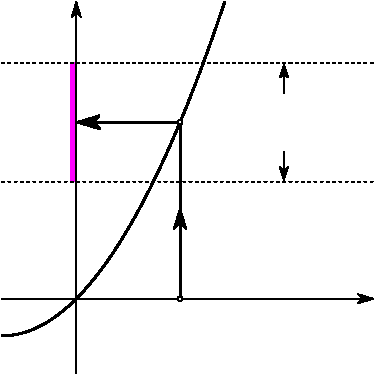
\includegraphics{03epsAndNoDelta.pdf}}
        \put( -2.00,  92.85){\sffamily\itshape \makebox[0pt][r]{$L-\varepsilon$}}
    \put( -2.00, 149.81){\sffamily\itshape \makebox[0pt][r]{$L+\varepsilon$}}
    \put( 31.60, 121.33){\sffamily\itshape \makebox[0pt][r]{$L$}}
    \put(108.24, 168.50){\sffamily\itshape $y=f(x)$}
    \put( 84.44,  24.60){\sffamily\itshape $a$}
    \put( 91.44, 121.33){\sffamily\itshape \
How close must $x$ be to $a$ for $f(x)$ to end up in this range?
}
\end{picture}


  
    \begin{picture} (180.000000,180.000000)(0,0)
    \put(0.0, 0.0){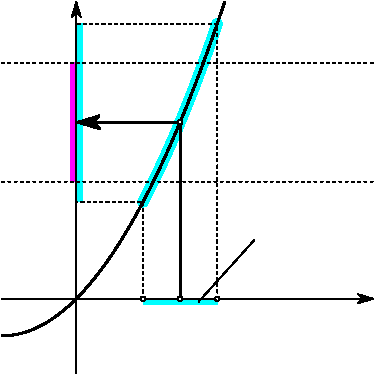
\includegraphics{03epsAndDeltaTooBig.pdf}}
        \put( -2.00,  92.85){\sffamily\itshape \makebox[0pt][r]{$L-\varepsilon$}}
    \put( -2.00, 149.81){\sffamily\itshape \makebox[0pt][r]{$L+\varepsilon$}}
    \put( 31.60, 121.33){\sffamily\itshape \makebox[0pt][r]{$L$}}
    \put(108.24, 168.50){\sffamily\itshape $y=f(x)$}
    \put(107.24,  39.60){\sffamily\itshape $a+\delta$}
    \put( 44.64,  39.60){\sffamily\itshape $a-\delta$}
    \put( 84.44,  24.60){\sffamily\itshape $a$}
    \put(125.04,  64.72){\sffamily\itshape \begin{minipage}{240pt}
        For some $x$ in this interval $f(x)$ is not between
        $L-\varepsilon$ and $L+\varepsilon$. Therefore the $\delta$ in this
        picture is too big for the given $\varepsilon$.  You need a smaller
        $\delta$.
        \end{minipage}}
\end{picture}


  
    \begin{picture} (180.000000,180.000000)(0,0)
    \put(0.0, 0.0){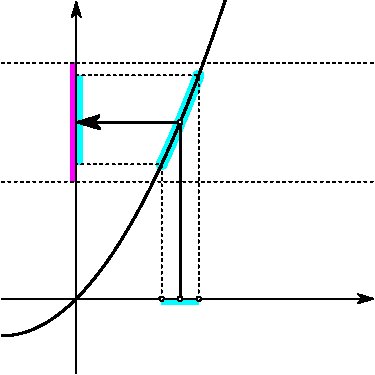
\includegraphics{03epsAndDelta.pdf}}
        \put( -2.00,  92.85){\sffamily\itshape \makebox[0pt][r]{$L-\varepsilon$}}
    \put( -2.00, 149.81){\sffamily\itshape \makebox[0pt][r]{$L+\varepsilon$}}
    \put( 31.60, 121.33){\sffamily\itshape \makebox[0pt][r]{$L$}}
    \put(108.24, 168.50){\sffamily\itshape $y=f(x)$}
    \put( 98.34,  39.60){\sffamily\itshape $a+\delta$}
    \put( 53.54,  39.60){\sffamily\itshape $a-\delta$}
    \put( 84.44,  24.60){\sffamily\itshape $a$}
\end{picture}

\end{figure}

\begin{figure}[t]
  \framebox{
    \begin{minipage}{0.95\textwidth} \sffamily \null \smallskip

      \centerline{\bfseries Propagation of errors -- another interpretation
        of $\varepsilon$ and $\delta$} \vbox to2pt{} According to the limit
      definition ``$\lim_{x\to R} \pi x^2 = A$'' is true if \textit{for
        every $\varepsilon>0$ you can find a $\delta>0$ such that $|x-R| <
        \delta$ implies $|\pi x^2 - A| < \varepsilon$.  } Here's a more
      concrete situation in which $\varepsilon$ and $\delta$ appear in
      exactly the same roles:

      \vbox to 2pt{}

      \begin{multicols}{2}\setlength{\parindent}{0pt}
      \setlength{\parindent}{2em}
      \noindent
      Suppose you are given a circle drawn on a piece of paper, and you
      want to know its area.  You decide to measure its radius, $R$,
      and then compute the area of the circle by calculating
      \[
      \textsf{Area} = \pi R^2.
      \]
      The area is a function of the radius, and we'll call that
      function $f$:
      \[
      f(x) = \pi x^2.
      \]

      When you measure the radius $R$ you will make an error, simply
      because you can never measure anything with infinite accuracy.
      Suppose that $R$ is the real value of the radius, and that $x$ is
      the number you measured.  Then the size of the error you made is
      \[
      \textsf{error in radius measurement} = |x-R|.
      \]
      When you compute the area you also won't get the exact value: you
      would get $f(x) = \pi x^2$ instead of $A = f(R) = \pi R^2$.  The
      error in your computed value of the area is
      \[
      \textsf{error in area } = |f(x) - f(R)| = |f(x) - A|.
      \]
      Now you can ask the following question:
      \begin{center}
        \itshape
        Suppose you want to know the area\\
        with an error of at most $\varepsilon$,\\
        then what is the largest error\\
        that you can afford to make\\
        when you measure the radius?
      \end{center}
      The answer will be something like this: if you want the computed
      area to have an error of at most $|f(x) - A| < \varepsilon$, then
      the error in your radius measurement should satisfy $|x-R| <
      \delta$.  You have to do the algebra with inequalities to compute
      $\delta$ when you know $\varepsilon$, as in the examples in this
      section.

      You would expect that if your measured radius $x$ is close enough
      to the real value $R$, then your computed area $f(x) = \pi x^2$
      will be close to the real area $A$.

      In terms of $\varepsilon$ and $\delta$ this means that you would
      expect that no matter how accurately you want to know the area
      (i.e., how small you make $\varepsilon$) you can always achieve
      that precision by making the error in your radius measurement
      small enough (i.e.  by making $\delta$ sufficiently small).
    \end{multicols}
    \vbox to2pt{}
  \end{minipage} }
\end{figure}

\subsection{Show that $\lim_{x\to 5}(2x+1)=11$ . } 
We have $f(x) = 2x+1$, $a=5$ and $L=11$, and the question we must answer is
``how close should $x$ be to $5$ if want to be sure that $f(x)=2x+1$
differs less than $\varepsilon$ from $L=11$?''

To figure this out we try to get an idea of how big $|f(x)-L|$ is:
\[
|f(x)-L| = \bigl|(2x+1)-11\bigr| = |2x-10| = 2\cdot |x-5| = 2\cdot |x-a|.
\]
So, if $2|x-a|<\varepsilon$ then we have $|f(x)-L|<\varepsilon$, i.e.,
\[
\text{if }|x-a|<\tfrac12\varepsilon \text{ then } |f(x)-L|<\varepsilon.
\]
We can therefore choose $\delta = \frac12\varepsilon$.  No matter what
$\varepsilon>0$ we are given our $\delta$ will also be positive, and if
$|x-5|<\delta$ then we can guarantee $|(2x+1) - 11|<\varepsilon$.  That
shows that $\lim_{x\to 5}2x+1 = 11$.




\subsection{The limit $\lim_{x\to 1}x^2 = 1$, the triangle inequality, and the ``don't choose $\delta>1$'' trick} 
This example will show you two basic tricks that are useful in many
$\varepsilon$-$\delta$ arguments.

The problem is to show that $x^2$ goes to 1 as $x$ goes to 1: we have $f(x) =
x^2$, $a=1$, $L=1$, and again the question is, ``how small should $|x-1|$ be to
guarantee $|x^2-1|<\varepsilon$?''

We begin by estimating the difference $|x^2-1|$
\[
|x^2-1| = |(x-1)(x+1)| = |x-1|\cdot|x+1|.
\]
How big can the two factors $|x-1|$ and $|x+1|$ be when we assume
$|x-1|<\delta$?  Clearly the first factor $|x-1|$ satisfies $|x-1|<\delta$
because that is what we had assumed.
\marginpar{\footnotesize\sffamily%
  The triangle inequality says that\\
  $|a+b|\leq |a| + |b|$\\
  for any two real numbers.}%
For the second factor we have
\[
|x+1| = \underbrace{|x-1 +2| \leq |x-1| + |2|}_{\text{by the triangle inequality}}
\leq \delta + 2.
\]
It follows that if $|x-1|<\delta$ then
\[
|x^2-1| \leq (2+\delta)\delta.
\]
Our goal is to show that if $\delta$ is small enough then the estimate on the
right will not be more than $\varepsilon$.  Here is the second trick in this
example: we agree \textit{that we always choose our $\delta$ so that $\delta\leq
1$.}  If we do that, then we will always have
\[
(2+\delta)\delta < (2+1)\delta =3\delta,
\]
so that $|x-1|<\delta$ with $\delta<1$ implies
\[
|x^2-1| < 3\delta.
\]
To ensure that $|x^2-1|<\varepsilon$, this calculation shows that we should
require $3\delta\leq \varepsilon$, i.e.\ we should choose $\delta \leq
\frac13\varepsilon$.  We must also live up to our promise never to choose
$\delta>1$, so if we are handed an $\varepsilon$ for which
$\frac13\varepsilon>1$, then we choose $\delta=1$ instead of $\delta =
\frac13\varepsilon$.  To summarize, we are going to choose
\[
\delta = \text{the smaller of }1\text{ and }\frac13\varepsilon.
\]
We have shown that for $\delta$ defined this way, then $|x-1|<\delta$
implies $|x^2-1|<\varepsilon$, no matter what $\varepsilon>0$ is.

The expression ``the smaller of $a$ and $b$'' shows up often, and is
abbreviated to $\min(a, b)$.  We could therefore say that in this problem
we will choose $\delta$ to be
\[
\delta = \min \bigl(1, \tfrac13 \varepsilon\bigr).
\]


\subsection{Show that $\lim_{x\to 4}1/x = 1/4$} 

We apply the definition with $a=4$, $L=1/4$ and $f(x) = 1/x$.
Thus, for any $\varepsilon>0$ we try to show that if $|x-4|$ is small
enough then one has $|f(x)-1/4|<\varepsilon$.

We begin by estimating $|f(x)-\frac14|$ in terms of $|x-4|$:
\[
|f(x)-1/4| = \left|\frac1x-\frac14\right| = \left| \frac{4-x}{4x}\right| =
\frac{|x-4|}{|4x|} =\frac{1}{|4x|}\,|x-4|.
\]
As before, things would be easier if $1/|4x|$ were a constant.  To achieve that
we again agree not to take $\delta>1$.  If we always have $\delta\leq 1$, then
we will always have $|x-4|<1$, and hence $3<x<5$.  How large can $1/|4x|$ be in
this situation?  Answer: the quantity $1/|4x|$ increases as you decrease $x$, so
if $3<x<5$ then it will never be larger than $1/|4\cdot 3| = \frac1{12}$.
We see that if we never choose $\delta>1$, we will always have
\[
|f(x) - \tfrac14|\leq \tfrac1{12}|x-4| \quad\text{for}\quad |x-4|<\delta.
\]
To guarantee that $|f(x)-\frac14|<\varepsilon$ we could therefore require
\[
\tfrac1{12} |x-4|<\varepsilon, \quad\text{i.e.}\quad |x-4| <12\varepsilon.
\]
Hence if we choose $\delta=12\varepsilon$ or any smaller number, then
$|x-4|<\delta$ implies $|f(x)-4|<\varepsilon$.  Of course we have to honor
our agreement never to choose $\delta>1$, so our choice of $\delta$ is
\[
\delta = \text{the smaller of }1\text{ and }12\varepsilon = \min \bigl(1,
12\varepsilon\bigr).
\]

\section{Problems} 
\problemfont 
\problem \groupproblem Joe offers to make square sheets of paper for 
Bruce.  Given $x>0$ Joe plans to mark off a length $x$ and cut out a
square of side $x$.  Bruce asks Joe for a square with area 4 square
foot.  Joe tells Bruce that he can't measure \emph{exactly} 2 feet and
the area of the square he produces will only be approximately 4 square
feet.  Bruce doesn't mind as long as the area of the square doesn't
differ more than $0.01$ square feet from what he really asked for
(namely, 4 square foot).

\subprob What is the biggest error Joe can afford to make when he
marks off the length $x$?

\subprob Jen also wants square sheets, with area $4$ square feet.
However, she needs the error in the area to be less than $0.00001$
square foot.  (She's paying.)

How accurately must Joe measure the side of the squares he's going to cut
for Jen?

\problem \groupproblem \textit{(Joe goes cubic.)}  Joe is offering to 
build cubes of side $x$.  Airline regulations allow you take a cube on
board provided its volume and surface area add up to less than $33$
(everything measured in feet).  For instance, a cube with 2-foot sides
has volume$+$area equal to $2^3 + 6\times 2^2 = 32$.

If you ask Joe to build a cube whose volume plus total surface area is
$32$ with an error of at most $\varepsilon$, then what error
can he afford to make when he measures the side of the cube he's
making?

\problem Our definition of a derivative in 
\eqref{eq:derivative-defined-first-time} contains a limit.  What is the
function ``$f$'' there, and what is the variable?
\answer 
The equation \eqref{eq:derivative-defined-first-time} already
contains a function $f$, but that is not the right function.  In
\eqref{eq:derivative-defined-first-time} $\Delta x$ is the variable,
and $g(\Delta x) = (f(x+\Delta x)-f(x))/\Delta x$ is the function; we
want $\lim_{\Delta x\to 0}g(\Delta x)$.
\endanswer
% !!! Issue: Almost all of these exercises are much harder than the problems in the section!
\begin{center}
  \it Use the $\varepsilon$--$\delta$ definition to prove the following limits:
\end{center}
\begin{multicols}{3}\setlength{\parindent}{0pt}

\problem \(\DS \lim_{x\to 1} 2x-4 = -2 \) 
\answer 
$\delta = \varepsilon/2$.
\endanswer

\problem \(\DS\lim_{x\to2} x^2 = 4\). 
\answer 
$\delta = \min \bigl\{1, \frac16\varepsilon\bigr\}$
\endanswer

\problem \(\DS \lim_{x\to 2} x^2-7x +3 = -7 \) 
\answer 
$|f(x) - (-7) |=|x^2-7x+10| = |x-2|\cdot|x-5| $.  If you choose
$\delta\leq 1$ then $|x-2|<\delta$ implies $1<x<3$, so that $|x-5|$
is at most $|1-5| = 4$.
So, choosing $\delta\leq 1$ we always have $|f(x) - L|<4|x-2|$ and
$|f(x) - L|<\varepsilon$ will follow from $|x-2|<\frac14\varepsilon$.
Our choice is then: $\delta = \min \bigl\{1, \frac14\varepsilon
\bigr\}$.
\endanswer

\problem \(\DS \lim_{x\to 3} x^3 = 27 \) 
\answer $f(x) = x^3$, $a=3$, $L=27$. 

When $x=3$ one has $x^3=27$, so $x^3-27=0$ for $x=3$.  Therefore you
can factor out $x-3$ from $x^3-27$ by doing a long division.  You get
$x^3-27 = (x-3)(x^2+3x+9)$, and thus
\[
|f(x) - L| = |x^3-27| =|x^2+3x+9|\cdot|x-3|.
\]
Never choose $\delta>1$.  Then $|x-3|<\delta$ will imply $2<x<4$ and
therefore
\[
|x^2+3x+9| \leq 4^2+3\cdot4+9 = 37.
\]
So if we always choose $\delta\leq 1$, then we will always have
\[
|x^3-27|\leq 37\delta \quad\text{for}\quad |x-3|<\delta.
\]
Hence, if we choose $\delta=\min\left\{ 1, \tfrac1{37}\varepsilon
\right\}$ then $|x-3|<\delta$ guarantees $|x^3-27| < \varepsilon$.


\endanswer

\problem \(\DS\lim_{x\to2} x^3 + 6x^2 = 32\). 

\problem \label{ex:03limitofsqrt4} 
$\DS \lim_{x\to4}\sqrt x = 2$.
\answer 
$f(x) = \sqrt x$, $a=4$, $L=2$.
You have
\[
\sqrt x - 2 = \frac{(\sqrt x-2)(\sqrt x +2)}{\sqrt x +2}
=\frac{x-4}{\sqrt x+2}
\]
and therefore
\begin{equation}\label{eq:03sol-fx-L-estimate}
  |f(x) - L | = \frac{1}{\sqrt x+2}|x-4|.
\end{equation}
Once again it would be nice if we could replace $1/(\sqrt x + 2)$ by
a constant, and we achieve this by always choosing $\delta\leq 1$.
If we do that then for $|x-4|<\delta$ we always have $3<x<5$ and
hence
\[
\frac{1}{\sqrt x+2} < \frac{1}{\sqrt 3 +2},
\]
since $1/(\sqrt x+ 2)$ increases as you decrease $x$.

So, if we always choose $\delta\leq 1$ then $|x-4|<\delta$ guarantees
\[
|f(x)-2| < \frac1{\sqrt3 +2}|x-4|,
\]
which prompts us to choose $\delta = \min\left\{ 1, (\sqrt
  3+2)\varepsilon \right\}$.

\textbf{A smarter solution:} We \emph{can} replace $1/(\sqrt x +2)$
by a constant in \eqref{eq:03sol-fx-L-estimate}, because for all $x$
in the domain of $f$ we have $\sqrt x \geq0$, which implies
\[
\frac1{\sqrt x+ 2} \leq \frac 12.
\]
Therefore $|\sqrt x- 2| \leq \frac12|x-4|$, and we could choose
$\delta = 2\varepsilon$.
\endanswer

\problem $\DS \lim_{x\to3}\sqrt{x+6} = 3$. 
\answer 
Hints:
\[
\sqrt{x+6}-3 = \frac{x+6-9}{\sqrt{x+6} + 3} = \frac{x-3}{\sqrt{x+6} +
  3}
\]
so
\[
|\sqrt{x+6} - 3|\leq \tfrac13 |x-3|.
\]
\endanswer

\problem $\DS \lim_{x\to 2}\frac{1+x}{4+x} = \tfrac12$. 
\answer 
We have
\[
\left|\frac{1+x}{4+x} - \frac{1}{2}\right| =
\left|\frac{x-2}{4+x}\right|.
\]
If we choose $\delta\le1$ then $|x-2|<\delta$ implies $1<x<3$ so that
\[
\underline{\frac17 <\;}{\text{we don't care}} \frac{1}{4+x} <
\frac15.
\]
Therefore
\[
\left|\frac{x-2}{4+x}\right| < \tfrac15 |x-2|,
\]
so if we want $|f(x) - \tfrac12| <\varepsilon$ then we must require
$|x-2|< 5\varepsilon$.  This leads us to choose
\[
\delta = \min\left\{ 1, 5\varepsilon \right\}.
\]
\endanswer

\problem $\DS \lim_{x\to 1}\frac{2-x}{4-x} = \tfrac13$. 

\problem $\DS \lim_{x\to 3}\frac{x}{6-x} = 1$. 

\problem \(\DS \lim_{x\to 0} \sqrt{|x|} = 0\) 
\end{multicols}


\noproblemfont
\section{Variations on the limit theme} 
\label{sec:variations-on-limit-theme}%
Not all limits are ``for $x\to a$''.  Here we describe some variations on the
concept of limit.

\subsection{Left and right limits. } 
When we let ``$x$ approach $a$'' we allow $x$ to be larger or smaller
than $a$, as long as $x$ ``gets close to $a$''.  If we explicitly want to study
the behavior of $f(x)$ as $x$ approaches $a$ through values larger than
$a$, then we write
\[
\lim_{x\searrow a} f(x)\text{ or } \lim_{x\to a+} f(x) \text{ or }
\lim_{x\to a+0} f(x) \text{ or } \lim_{x\to a, x>a} f(x).
\]
All four notations are commonly used.  Similarly, to designate the value which
$f(x)$ approaches as $x$ approaches $a$ through values below $a$ one writes
\[
\lim_{x\nearrow a} f(x)\text{ or } \lim_{x\to a-} f(x) \text{ or }
\lim_{x\to a-0} f(x) \text{ or } \lim_{x\to a, x<a} f(x).
\]
The precise definition of these ``one-sided'' limits goes like this:

\subsection{Definition of right-limits} 
\itshape
Let $f$ be a function.  Then
\begin{equation}\label{eq:one-sided-lim-formulation}
  \lim_{x\searrow a} f(x) = L.
\end{equation}
means that for every $\varepsilon>0$ one can find a $\delta>0$ such that
\[
a<x<a+\delta \implies |f(x)-L|<\varepsilon
\]
holds for all $x$ in the domain of $f$.  \upshape
\subsection{Definition of left-limits} 
\itshape
Let $f$ be a function.  Then
\begin{equation}\label{eq:left-sided-lim-formulation}
  \lim_{x\nearrow a} f(x) = L.
\end{equation}
means that for every $\varepsilon>0$ one can find a $\delta>0$ such that
\[
a-\delta<x<a \implies |f(x)-L|<\varepsilon
\]
holds for all $x$ in the domain of $f$.  \upshape
The following
theorem tells you how to use one-sided limits to decide if a function
$f(x)$ has a limit at $x=a$.

\subsection{Theorem}\label{one_sided_limit_thm} 
\itshape%
The two-sided limit $\displaystyle \lim_{x\to a} f(x)$
exists if and only if the two one-sided limits
\[
  \lim_{x\searrow a} f(x), \quad\text{and}\quad \lim_{x\nearrow a} f(x)
\]
exist and have the same value.
\upshape

\subsection{Limits at infinity} 
Instead of letting $x$ approach some finite number, one can let $x$ become
``larger and larger'' and ask what happens to $f(x)$.  If there is a number
$L$ such that $f(x)$ gets arbitrarily close to $L$ if one chooses $x$
sufficiently large, then we write
\[
\lim_{x\to \infty} f(x) = L
\]
(``The limit for $x$ going to infinity is $L$.'')
We have an analogous definition for what happens to $f(x)$ as $x$ becomes very
large and negative: we write
\[
\lim_{x\to -\infty} f(x) = L
\]
(``The limit for $x$ going to negative infinity is $L$.'')
  
% Shouldn't we include the actual epsilon definition??
% Yes, we should.  
Here are the precise definitions:
\itshape
Let $f(x)$ be a function which is defined on an interval $x_0<x<\infty$.
If there is a number $L$ such that for every $\varepsilon>0$ we can find
an $A$ such that
\[
x>A \implies |f(x) - L| <\varepsilon
\]
for all $x$, then we say that the limit of $f(x)$ for $x\to\infty$ is $L$.
\upshape
\itshape
Let $f(x)$ be a function which is defined on an interval $-\infty < x < x_0$.
If there is a number $L$ such that for every $\varepsilon>0$ we can find
an $A$ such that
\[
x<-A \implies |f(x) - L| <\varepsilon
\]
for all $x$, then we say that the limit of $f(x)$ for $x\to\infty$ is $L$.
\upshape
These definitions are very similar to the original definition of the limit.
Instead of $\delta$ which specifies how close $x$ should be to $a$, we now
have a number $A$ that says how large $x$ should be, which is a way of
saying ``how close $x$ should be to infinity'' (or to negative infinity).

\begin{figure}[ht]
  \centering
  
    \begin{picture} (360.000000,134.592593)(0,0)
    \put(0.0, 0.0){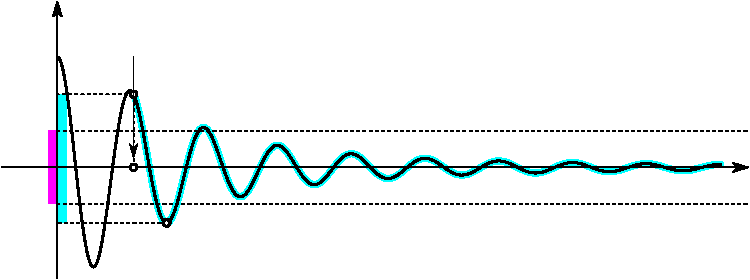
\includegraphics{03ftozeroAtoosmall.pdf}}
        \put( 64.11, 109.07){\sffamily\itshape \makebox[0pt][c]{$A$}}
    \put(  9.52,  68.54){\sffamily\itshape $+\varepsilon$}
    \put(  9.52,  33.53){\sffamily\itshape $-\varepsilon$}
    \put(186.63, 107.07){\sffamily\itshape \makebox[0pt][l]{%
\parbox{2in}{\centering Here $A$ is too small, because\\
 $f(x) > \varepsilon$ happens for some $x\geq A$}}}
\end{picture}


  
    \begin{picture} (360.000000,134.592593)(0,0)
    \put(0.0, 0.0){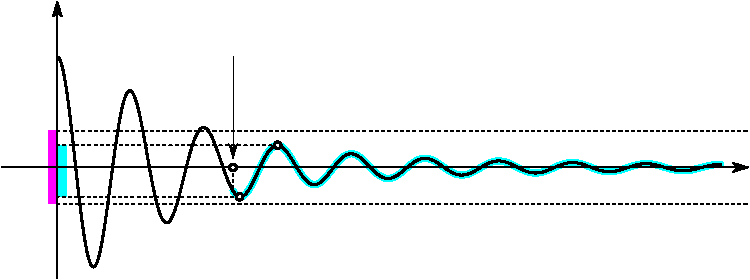
\includegraphics{03ftozeroAok.pdf}}
        \put(111.85, 109.07){\sffamily\itshape \makebox[0pt][c]{$A$}}
    \put(  9.52,  68.54){\sffamily\itshape $+\varepsilon$}
    \put(  9.52,  33.53){\sffamily\itshape $-\varepsilon$}
    \put(186.63, 107.07){\sffamily\itshape \makebox[0pt][l]{%
\parbox{2in}{\centering This $A$ is large enough, because\\
 $f(x)$ is in the right range\\
for all $x\geq A$}}}
\end{picture}

  \caption{The limit of $f(x)$ as $x\to\infty$; how large must $x$ be
    if you need $-\varepsilon < f(x) < \varepsilon$?}
  \label{fig:limit-of-xinv-at-infty}
\end{figure}
\subsection{Example -- Limit of $1/x$} 
\label{ex:lim1overx-at-infty-proved}
The larger $x$ is, the smaller its reciprocal is, so it seems natural that $1/x
\to 0$ as $x\to \infty$.  To \emph{prove} that $\lim_{x\to\infty}1/x = 0$ we
apply the definition to $f(x) = 1/x$, $L=0$.

For a given $\varepsilon>0$, we need to show that
\begin{equation}\label{eq:1overx-small-for-x-large}
  \left|\frac1x - L\right|<\varepsilon \text{ for all } x>A
\end{equation}
provided we choose the right $A$.

How do we choose $A$?  $A$ is not allowed to depend on $x$, but it may
depend on $\varepsilon$.

Let's decide that we will always take $A>0$, so that we only need consider
positive values of $x$.  Then \eqref{eq:1overx-small-for-x-large} simplifies to
\[
\frac 1x<\varepsilon
\]
which is equivalent to
\[
x>\frac1\varepsilon.
\]
This tells us how to choose $A$.  Given any positive $\varepsilon$, we will
simply choose
\[
  A= \text{ the larger of } 0 \text{ and } \frac1\varepsilon
\]
Then we have $|\frac1x-0| = \frac1x <\varepsilon$ for all $x>A$, so we
have proved that $\lim_{x\to\infty}1/x=0$.


\section{Properties of the Limit} 
\label{sec:limitProperties}%
The precise definition of the limit is not easy to use, and
fortunately we don't need to use it very often.  Instead, there
are a number of properties that limits possess that will allow us to compute
complicated limits without having to resort to ``epsiloncy.''

The following properties also apply to the variations on the limit from
\S\ref{sec:variations-on-limit-theme}.  I.e., the following statements remain
true if one replaces each limit by a one-sided limit, or a limit for
$x\to\infty$.  \smallskip

\textbf{Limits of constants and of $x$. } If $a$ and $c$ are constants,
then
\begin{equation}
  \lim_{x\to a}c=c \tag{$P_1$}
\end{equation}
and
\begin{equation}
  \lim_{x\to a} x= a.\tag{$P_2$}
\end{equation}

\textbf{Limits of sums, products, powers, and quotients. } Let $F_1$ and $F_2$ be
two given functions whose limits for $x\to a$ we know,
\[
\lim_{x\to a}F_1(x)=L_1, \qquad \lim_{x\to a}F_2(x)=L_2.
\]
Then
\begin{align*}
  \lim_{x\to a}\bigl(F_1(x)+F_2(x)\bigr) &= L_1+L_2, \tag{$P_3$} \\
  \lim_{x\to a}\bigl(F_1(x)-F_2(x)\bigr) &= L_1 - L_2, \tag{$P_4$} \\
  \lim_{x\to a}\bigl(F_1(x)\cdot F_2(x)\bigr) &= L_1\cdot L_2 . \tag{$P_5$} \\
\end{align*}
If $ \lim_{x\to a}F_2(x)\ne0$, then
\begin{equation}
  \lim_{x\to a}\frac{F_1(x)}{F_2(x)}= \frac{L_1}{L_2}.\tag{$P_6$}
\end{equation}
Finally, if $k$ is an integer, then
\begin{equation}
\lim_{x\to a}\bigl(F_1(x)^k\bigr) = L_1\,^k . \tag{$P_{7}$}
\end{equation}
If $L_1 > 0$, then $(P_7)$ holds for any real number $k$.

In other words ``the limit of the sum is the sum of the limits,'' etc.  One can
prove these laws using the definition of limit in
\S\ref{sec:formal-limit-def} but we will not do this here.  However, these laws
should seem like common sense: if, for $x$ close to $a$, the quantity
$F_1(x)$ is close to $L_1$ and $F_2(x)$ is close to $L_2$, then certainly
$F_1(x)+F_2(x)$ should be close to $L_1+L_2$. (And so forth.)



Later in this chapter we will add two more properties of limits to
this list.  They are the ``Sandwich Theorem''
(\S\ref{sec:limits-and-inequalities}) and the substitution theorem
(\S\ref{sec:continuity}).

\section{Examples of limit computations} 

\subsection{Find $\lim_{x\to2}x^2$} 
We have
\begin{align*}
  \lim_{x\to2} x^2 &= \lim_{x\to2} x\cdot x \\
  &= \bigl( \lim_{x\to2} x\bigr)\cdot \bigl( \lim_{x\to2} x\bigr)
  &\text{by $(P_5)$}\\
  &= 2\cdot 2 = 4.
\end{align*}
Similarly,
\begin{align*}
  \lim_{x\to2} x^3 &= \lim_{x\to2} x\cdot x^2 \\
  &= \bigl( \lim_{x\to2} x\bigr)\cdot \bigl( \lim_{x\to2} x^2\bigr)
  &\text{$(P_5)$ again}\\
  &= 2\cdot 4 = 8,
\end{align*}
and, by $(P_4)$
\[
\lim_{x\to2} x^2-1 = \lim_{x\to2} x^2 - \lim_{x\to2} 1 = 4-1 = 3,
\]
and, by $(P_4)$ again,
\[
\lim_{x\to2} x^3-1 = \lim_{x\to2} x^3 - \lim_{x\to2} 1 = 8-1 = 7,
\]
Putting all this together, we get
\[
\lim_{x\to 2}\frac{x^3-1}{x^2-1} = \frac{2^3-1}{2^2-1} = \frac{8-1}{4-1}=
\frac{7}{3}
\]
because of $(P_6)$.  To apply $(P_6)$ we must check that the denominator
(``$L_2$'') is not zero.  Since the denominator is 3 everything is OK, and
we were allowed to use $(P_6)$.


\subsection{Try the examples \ref{ex:limit-by-sub-good} and \ref{ex:limit-by-sub-bad} using the limit properties} 
To compute $\lim_{x\to 2}(x^2-2x)/(x^2-4)$ we first use the limit
properties to find
\[
\lim_{x\to2} x^2-2x = 0 \text{ and }\lim_{x\to 2}x^2 - 4 = 0.
\]
to complete the computation we would like to apply the last property
$(P_6)$ about quotients, but this would give us
\[
\lim_{x\to2} f(x) = \frac 00.
\]
The denominator is zero, so we were not allowed to use $(P_6)$ (and the
result doesn't mean anything anyway).  We have to do something else.

The function we are dealing with is a \emph{rational function}, which means
that it is the quotient of two polynomials.  For such functions there is an
algebra trick that always allows you to compute the limit even if you
first get $\frac 00$.  The thing to do is to divide numerator and
denominator by $x-2$.  In our case we have
\[
x^2-2x = (x-2)\cdot x, \qquad x^2-4 = (x-2)\cdot (x+2)
\]
so that
\[
\lim_{x\to2} f(x) =\lim_{x\to2} \frac{(x-2)\cdot x } {(x-2)\cdot (x+2)} =
\lim_{x\to2} \frac{x}{x+2}.
\]
After this simplification we \emph{can} use the properties $(P_{\ldots})$
to compute
\[
\lim_{x\to2} f(x) = \frac{2}{2+2} = \frac12.
\]

\subsection{Example -- Find $\lim_{x\to 2}\sqrt x$} 
\label{ex:limit-of-sqrt-at-2}
  We can apply limit property $(P_{5a})$ with $k=1/2$ to see that
\[
  \lim_{x\to2} \sqrt{x} = \lim_{x\to2} x^{1/2} = [\lim_{x\to2} x]^{1/2} =
  2^{1/2} = \sqrt{2}.
\]

\subsection{Example -- The derivative of $\sqrt x$ at $x=2$} 
Find
\[
\lim_{x\to2}\frac{\sqrt x-\sqrt2}{x-2}
\]
assuming the result from the previous example (i.e., assuming that
$\lim_{x\to2}\sqrt x = \sqrt2$.)

\textit{Solution: } The function is a fraction whose numerator and
denominator vanish when $x=2$, so the limit is of the form ``$\frac00$''.
We use an algebra trick; namely, multiplying the numerator and
denominator by $\sqrt{x}+\sqrt{2}$:
\[
\frac{\sqrt x-\sqrt2}{x-2}
= \frac{(\sqrt x-\sqrt2)(\sqrt{x}+\sqrt{2})}{(x-2)(\sqrt
  x+\sqrt2)} =\frac{1}{\sqrt x+\sqrt2}.
\]
Now we can use the limit properties to compute
\[
\lim_{x\to2} \frac{\sqrt x-\sqrt 2}{x-2} = \lim_{x\to2} \frac{1}{\sqrt
  x+\sqrt 2} =\frac1{2\sqrt2} =\frac{\sqrt2}4.
\]



\subsection{Limit as $x\to\infty$ of Rational Functions} 
\label{sec:lim-at-infty-of-rationalfunction}%
A rational function is the quotient of two polynomials:
\begin{equation}\label{eq:your-typical-rational-function}
  R(x) = \frac{a_nx^n+\cdots +a_1x+a_0}{b_mx^m+\cdots+b_1x+b_0}.
\end{equation}
We have seen that
\[
\lim_{x\to\infty} \frac 1x =0
\]
We even proved this in example \ref{ex:lim1overx-at-infty-proved}.  Using
this we can find the limit at $\infty$ for any rational function $R(x)$ as
in \eqref{eq:your-typical-rational-function}.  We could turn the outcome
of the calculation of $\lim_{x\to\infty}R(x)$ into a boxed recipe
involving the degrees $n$ and $m$ of the numerator and denominator, and
also their coefficients $a_i$, $b_j$, which you, the student, would then memorize,
but it is better to remember {\itshape the trick:}
\begin{verse}\itshape
  To find the limit as $x\to\infty$,\\
  of some rational function you have been given,\\
  factor the highest occurring powers of $x$,\\
  both from numerator and from denominator.
\end{verse}
For example, let's compute
\[
\lim_{x\to\infty}\frac{3x^2+3}{5x^2+7x-39}.
\]
Remember the trick and factor $x^2$ from top and bottom. You get
\begin{align*}
  \lim_{x\to\infty}\frac{3x^2+3}{5x^2+7x-39}
  &= \lim_{x\to\infty}\frac{x^2}{x^2} \; \frac{3+3/x^2}{5+7/x-39/x^2}
  & \text{(algebra)}\\
  &= \lim_{x\to\infty}\frac{3+3/x^2}{5+7/x-39/x^2}& \text{(more algebra)}\\
  &= \frac{\lim_{x\to\infty}(3+3/x^2)}{\lim_{x\to\infty}(5+7/x-39/x^2)}
  &\text{(limit properties)}\\
  &= \frac35.
\end{align*}
At the end of this computation, we used the limit properties
$(P_\ast)$ to break the limit down into simpler pieces like
$\lim_{x\to\infty}39/x^2$, which we can directly evaluate; for example, we have
\[
\lim_{x\to\infty} 39/x^2 =\lim_{x\to\infty} 39\cdot \left( \frac1x
\right)^2 = \left( \lim_{x\to\infty}39\right)\cdot \left(
  \lim_{x\to\infty}\frac1x \right)^2 = 39 \cdot 0^2 =0.
\]
  The other terms are similar.
  
  
\subsection{Another example with a rational function} 
Compute
\[
\lim_{x\to\infty} \frac {2x}{4x^3+5}.
\]
We apply ``the trick'' again and factor $x$ out of the numerator and
$x^3$ out of the denominator.
This leads to
\begin{align*}
  \lim_{x\to\infty} \frac {2x}{4x^3+5}
  &=\lim_{x\to\infty} \Bigl(\frac{x}{x^3}\;\frac{2}{4+5/x^3}\Bigr)\\
  &=\lim_{x\to\infty} \Bigl(\frac{1}{x^2}\;\frac{2}{4+5/x^3}\Bigr)\\
  &=\lim_{x\to\infty} \Bigl(\frac{1}{x^2}\Bigr)\cdot \Bigl(\lim_{x\to\infty}\frac{2}{4+5/x^3}\Bigr)\\
  &=0\cdot \tfrac24\\
  &=0.
\end{align*}
This example and the previous cover two of the three possible
combinations of degrees $n$ and $m$, namely $n=m$ and $n<m$.  To show
the remaining case, in which the numerator has higher degree than the
denominator, we should do yet another example, but that one will have
to wait a few pages (see
\S~\ref{sec:03infinite-limit-of-rational-functions})


\section{When limits fail to exist} 
In the last couple of examples we worried about the possibility that a
limit $\lim_{x\to a}g(x)$ actually might not exist.  This can actually
happen, and in this section we'll see a few examples of what failed limits
look like.  First let's agree on what we will call a ``failed limit.''

\subsection{Definition} 
\itshape
If there is no number $L$ such that $\lim_{x\to a}f(x) = L$, then we say
that the limit $\lim_{x\to a}f(x)$ does not exist.  \upshape


\subsection{The sign function near $x=0$} 
\label{sec:sign-function-has-no-limit}
The ``sign function'' is defined by%
\marginpar{\footnotesize\sffamily\raggedleft 
    \begin{picture} (90.000000,42.228571)(0,0)
    \put(0.0, 0.0){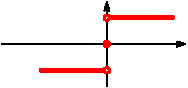
\includegraphics{03signOFx.pdf}}
        \put( 48.29,  31.69){\sffamily\itshape \makebox[0pt][r]{$1$}}
    \put( 53.29,   6.54){\sffamily\itshape \makebox[0pt][l]{$-1$}}
\end{picture}
\\[1ex]
  $y=\sign(x)\hfill\null$\\
  There are those who do not like the notation
  ``$\sign(x)$,'' and prefer to write\\
  $g(x) = \frac{x}{|x|}$
  instead of $g(x) = \sign(x)$.  If you think about this formula for a
  moment you'll see that $\sign(x)$ and $ x/|x|$ are the same for all
  $x\neq0$.  When $x=0$ the quotient $x/|x|$ is of course not defined.
}%
\[
\sign (x) =
\begin{cases}
  -1 & \text{for $x<0$}\\ 0 & \text{for $x=0$}\\ 1 & \text{for $x>0$}
\end{cases}
\]
Note that ``the sign of zero'' is defined to be zero.  Our question is: does the
sign function have a limit at $x=0$?  The answer is \emph{no}, and here is why:
since $\sign(x) = +1$ for all positive values of $x$, we see that
\[
 lim_{x\searrow 0} \sign(x) = +1.
\]
Similarly, since $\sign(x) = -1$ for all negative values of $x$, we see that
\[
 lim_{x\nearrow 0} \sign(x) = -1.
\]
 Then by the result of \ref{one_sided_limit_thm}, we see that because the two one-sided limits have different values, the two-sided limit does not exist.  (Essentially, if the two-sided limit existed, then it would have to be equal to both $+1$ and $-1$ at the same time, which is impossible.)
\[
\text{Conclusion:}\quad
\lim_{x\to 0} \sign (x) \text{ does not exist.}
\]
\subsection{The example of the backward sine} 
\label{sec:03backward-sine}
Contemplate the limit as $x\to0$ of the ``backward sine,'' i.e.
\[
\lim_{x\to 0}\sin \Bigl(\frac\pi x\Bigr).
\]

When $x=0$ the function $f(x)=\sin(\pi /x)$ is not defined, because its
definition involves division by $x$.  What happens to $f(x)$ as $x\to0$?
First, $\pi /x$ becomes larger and larger (``goes to infinity'') as
$x\to0$.  Then, taking the sine, we see that $ \sin(\pi /x)$ oscillates
 between $+1$ and $-1$ infinitely often as $x\to0$, since, for example, we can calculate that $f(\frac{2}{4k+1})=+1$ and $f(\frac{2}{4k+3})=-1$ for each integer $k$. This means that $f(x)$
gets close to any number between $-1$ and $+1$ as $x\to0$, but that the
function $f(x)$ \emph{never stays close} to any particular value because it
keeps oscillating up and down between $+1$ and $-1$.

\begin{figure}[ht]\centering
  \input ../figures/221/03sinePiOverx.tex
  \caption{Graph of $y = \sin\frac\pi x$ for $-3<x<3$,\ \ $x\neq0$.}
  \label{fig:03sinePiOverx}
\end{figure}

Here again, the limit $\lim_{x\to0}f(x)$ does not exist.  We have arrived
at this conclusion by only considering what $f(x)$ does for small positive
values of $x$.  So the limit fails to exist in a stronger way than in the
example of the sign-function. There, even though the limit didn't exist,
the one-sided limits existed.  In the present example we see that even the
one-sided limits
\[
  \lim_{x\searrow 0} \sin \Bigl(\frac{\pi}{x} \Bigr)
  \text{ and }
  \lim_{x\nearrow 0} \sin \Bigl(\frac{\pi}{x} \Bigr)
\]
do not exist.
\subsection{Limit properties for limits that don't exist} 
The limit properties all say that some limit exists (and what it's equal to),
but by applying some logic you can sometimes also use the limit properties to
conclude that a limit does \emph{not} exist.  For instance:
\subsection*{Theorem}% lim g+h doesn't exist implies either limg or limh fails 
\itshape
If $\lim_{x\to a}f(x) + g(x)$ does not exist, then at least one of the
two limits $\lim_{x\to a}f(x)$ or $\lim_{x\to a}g(x)$ does not exist.
\upshape\medskip
\noindent%
In English: ``if the sum of two functions has no limit, then one of
the terms also has no limit.''
This follows directly from Property $(P_3)$ which says that if $\lim
f(x)$ and $\lim g(x) $ both exist then $\lim f(x)+g(x)$ also must
exist.
\section{Limits that equal $\infty$} 
\label{sec:03limits-that-equal-infty}
For some limits that don't exist, we can be more descriptive about the
reason that the limit doesn't exist.  Here are some examples.

\subsection{The limit of $1/x$ at $x=0$} 
\label{sec:limit-1x-at-zero}
Consider the limit
\[
\lim_{x\to 0} \frac{1} {x}.
\]
As $x$ decreases to $x=0$ through smaller and smaller positive values,
its reciprocal $1/x$ becomes larger and larger.  We say that instead
of going to some finite number, the quantity $1/x$ ``goes to
infinity'' as $x\searrow0$.  In symbols:
\begin{equation}
  \lim_{x\searrow 0} \frac{1} {x} = \infty.
  \label{eq:03limit-invx-is-infty}  
\end{equation}%
\marginpar{\input ../figures/221/03inverse-of-x.tex }%
Likewise, as $x$ approaches $0$ through negative numbers, its
reciprocal $1/x$ drops lower and lower, and we say that $1/x$ ``goes
to $-\infty$'' as $x\nearrow 0$.  Symbolically,
\begin{equation}
  \label{eq:03limit-invx-is-neg-infty}
    \lim_{x\nearrow 0} \frac{1} {x} = -\infty.
\end{equation}
The limits \eqref{eq:03limit-invx-is-infty} and
\eqref{eq:03limit-invx-is-neg-infty} are not like the normal limits we
have been dealing with so far.  Namely, when we write something like
\[
\lim_{x\to2} x^2 = 4
\]
we mean that the limit actually exists and that it is equal to $4$.
On the other hand, since we have agreed that $\infty$ is not a number,
the meaning of \eqref{eq:03limit-invx-is-infty} cannot be to say that
``the limit exists and its value is $\infty$.''

Instead, when we write
\begin{equation}
  \lim_{x\to a} f(x) = \infty
  \label{eq:03limit-of-f-infty}
\end{equation}
for some function $y=f(x)$, we mean, \emph{by definition,} that the
limit of $f(x)$ does not exist, and that it fails to exist in a
specific way: as $x\to a$, the value of $f(x)$ becomes ``larger and
larger,'' and in fact eventually becomes larger than any finite
number.

The language in that last paragraph shows you that this is an
intuitive definition, at the same level as the first definition of
limit we gave in \S\ref{sec:informal-limit-def}.  It contains the
usual suspect phrases such as ``larger and larger,'' or ``finite
number'' (as if there were any other kind.)  A more precise definition
involving epsilons can be given, but in this course we will not go
into this much detail.  As a final comment on infinite limits, it is
important to realize that, since \eqref{eq:03limit-of-f-infty} is not
a normal limit \emph{you cannot apply the limit rules to infinite
  limits. }  Here is an example of what goes wrong if you try anyway.

\subsection{Trouble with infinite limits} 
\label{sec:trouble-with-infinite-limits}
If you apply the limit properties to $\lim_{x\searrow0} 1/x = \infty$,
then you could conclude
\[
1 = \lim_{x\searrow 0} x\cdot \frac{1} {x}
 = \lim_{x\searrow 0} x \times \lim_{x\searrow 0}  \frac{1} {x}
 = 0 \times \infty
 = 0,
\]
because ``anything multiplied with zero is zero.''

After using the limit properties in combination with this infinite
limit we reach the absurd conclusion that $1=0$.  The moral of this
story is that you can't use the limit properties when some of the
limits are infinite.
% !!! Issue: This discussion of algebraic properties of infinite limits needs to
% be redone. It is extremely wrong not to explain why 2 times infinity is
% infinity. What should be done is to say the limit rules do hold, except that 0
% times infinity, infinity minus infinity, 0/0, and infinity / infinity are
% undefined. This would also fix the massive problems with the next example
% about rational functions.
\subsection{Limit as $x\to\infty$ of rational functions, again} 
\label{sec:03infinite-limit-of-rational-functions}
In \S~\ref{sec:lim-at-infty-of-rationalfunction} we computed the
limits of rational functions $R(x) = \frac{P(x)} {Q(x)}$ as
$x\to\infty$ in all cases where the degree of the numerator $P$ was
not more than the degree of the denominator $Q$.  Here we complete the
story by looking at the remaining case where $\deg P > \deg Q$.
We'll do the following examples:
\[
  A = \lim_{x\to\infty} x, \quad
  B = \lim_{x\to\infty} -7x^2, \quad
  C = \lim_{x\to\infty} \frac{x^3-2x} {1+25x^2}.
\]
The first limit is the easiest: ``as $x$ goes to infinity, $x$ goes to
infinity.''  So we have
\[
A = \lim_{x\to\infty} x = \infty.
\]
Remember, we don't have a precise definition that says when a limit
equals ``$\infty$,'' so we can't prove this here.  On the other hand,
if someone were to come up with a definition of the above limit that
would make it equal to something else, we would ask them to change
their definition instead of changing our mind about $\lim_{x\to\infty}
x$.
The second limit is only slightly harder: as $x\to\infty$, the square
$x^2$ also becomes arbitrarily large, and thus $-7x^2$ will go to
$-\infty$.  So we'll say  $B=-\infty$.
Finally, let's look at $C$.  We apply the trick from
\S~\ref{sec:lim-at-infty-of-rationalfunction}:
\[
C = \lim_{x\to\infty}  \frac{x^3-2x} {1+25x^2}
=  \lim_{x\to\infty} \frac{x^3} {x^2}  \frac{1-\frac2x} {\frac1x+25}.
\]
At this point we would like to use the limit properties to say
\[
C =  \lim_{x\to\infty} \frac{x^3} {x^2}  \frac{1-\frac2x} {\frac1x+25}
= \lim_{x\to\infty} \frac{x^3} {x^2}\; \lim_{x\to\infty}
\frac{1-\frac2x} {\frac1x+25}
=\bigl(\lim_{x\to\infty} x\bigr) \cdot \frac{1} {25}
=\infty \cdot \frac{1} {25}
=\infty.
\]
Unfortunately, as we have just seen, the limit properties are
unreliable when infinite limits are involved, so we have no
justification for using them here.  Nevertheless, the answer we got
this time seems reasonable; in an attempt to make it look more
reasonable you could write it this way:
\[
\frac{x^3} {x^2}  \frac{1-\frac2x} {\frac1x+25}
=x\cdot \frac{1-\frac2x}{\frac1x+25}
\approx x \cdot \frac{1} {25}
\]
for large $x$.  Therefore, as $x\to\infty$ the fraction
\[
\frac{x^3} {x^2}  \frac{1-\frac2x} {\frac1x+25}
\approx x \cdot \frac{1} {25}
\to\infty.
\]
% !!! Issue: This is also really bad style: what does "approximately equals"
% even mean here?!?
\section{What's in a name? -- Free Variables and Dummy variables} 
  % !!! Discuss: Should this section appear earlier, right near the definition of limit?
\label{sec:free-versus-dummy-variables}%
There is a big difference between the variables $x$ and $a$ in the formula
\[
\lim_{x\to a} 2x+1,
\]
namely $a$ is a \emph{free variable}, while $x$ is a \emph{dummy variable}
(or ``placeholder'' or a ``bound variable.'')

The difference between these two kinds of variables is this:
\begin{itemize}
\item if you replace a dummy variable in some formula consistently by some
  other variable then the value of the formula does not change.  On the
  other hand, it never makes sense to substitute a number for a dummy
  variable.

\item the value of the formula may depend on the value of the free
  variable.
\end{itemize}
To understand what this means consider the example $\lim_{x\to a}2x+1$
again.  The limit is easy to compute:
\[
\lim_{x\to a}2x+1 = 2a+1.
\]
If we replace $x$ by, say $u$ (systematically) then we get
\[
\lim_{u\to a} 2u+1
\]
which is again equal to $2a+1$.  This computation says that \textit{if some
  number gets close to $a$ then two times that number plus one gets close
  to $2a+1$.}  This is a very wordy way of expressing the formula, and you
can shorten things by giving a name (like $x$ or $u$) to the number that
approaches $a$.  But the result of our computation shouldn't depend on the
name we choose: it doesn't matter if we call it $x$ or $u$, or anything else.
Some prefer to call $x$ a bound variable, meaning that in
\[
\lim_{x\to a} 2x+1
\]
the $x$ in the expression $2x+1$ is bound to the $x$ written underneath the
limit -- you can't change one without changing the other.

Substituting a number for a dummy variable usually leads to complete
nonsense.  For instance, let's try setting $x=3$ in our limit: what is
\[
\lim_{3\to a}2\cdot 3+1\,?
\]
Of course $2\cdot 3+1 = 7$, but what does $7$ do when $3$ gets closer and
closer to the number $a$?  That's a silly question, because 3 is a constant
and it doesn't ``get closer'' to some other number like $a$!  (If you ever
see 3 get closer to another number then it's time to take a vacation!)

On the other hand the variable $a$ is free: you can assign it particular
values, and its value will affect the value of the limit.  For instance, if
we set $a=3$ (but leave $x$ alone), then we get
\[
\lim_{x\to 3} 2x+1
\]
and there's nothing strange about that, since the limit is $2\cdot3+1=7$ (no
problem).  We could substitute other values of $a$ and we would get
different answers. In general you get $2a+1$.

\section{Limits and Inequalities} 
\label{sec:limits-and-inequalities}%
This section has two theorems that let you compare limits of different
functions.  The properties in these theorems are not formulas that
allow you to compute limits like the properties $(P_1)$\ldots$(P_6)$
from \S\ref{sec:limitProperties}.  Instead, they allow us to
\emph{reason} about limits.

The first theorem should not surprise you --- all it says is that bigger
functions have bigger limits.

\subsection{Theorem} 
\itshape
Let $f$ and $g$ be functions whose limits as $x\to a$ exist, and assume
that $f(x)\leq g(x)$ holds for all $x$.  Then
\[
\lim_{x\to a}f(x) \leq \lim_{x\to a} g(x).
\]
\upshape

A useful special case arises when we set $f(x)=0$.  The theorem then says
that if a function $g$ never has negative values, then its limit will also
never be negative.
Here is the second theorem about limits and inequalities.

\subsection{The Sandwich Theorem} 
\itshape
Suppose that
\[
f(x)\le g(x)\le h(x)
\]
(for all $x$) and that both the limits
\[
  \lim_{x\to a} f(x) \text{ and } \lim_{x\to a} h(x)
\]
exist and are equal to the same value $L$. Then
\[
\lim_{x\to a} g(x)
\]
also exists and is equal to $L$.
\upshape

The theorem is useful when we want to know the limit of $g$, and when we
can \emph{sandwich} it between two functions $f$ and $h$ whose limits are
easier to compute.  The Sandwich Theorem looks like the first theorem of
this section, but there is an important difference: in the Sandwich Theorem
we don't have to assume that the limit of $g$ exists.  The inequalities
$f\leq g\leq h$ combined with the circumstance that $f$ and $h$ have the
same limit are enough to guarantee that the limit of $g$ exists.

\begin{figure}[h]\centering
  \input ../figures/221/03backwardCosSandwich.tex
  \caption{The graph of  $x\cos\frac\pi x$ is ``sandwiched'' in
    between the graphs of $y=+|x|$ and of $y=-|x|$.}
  \label{fig:03backwardCosSandwich}
\end{figure}

\subsection{Example: a Backward Cosine Sandwich. }
\label{sec:backward-cosine-sandwich}
  % Why wouldn't we use sine, because that's what we did earlier ?!?!?
\label{sec:03xcos1overx} The Sandwich Theorem says that if the function
$g(x)$ is sandwiched between two functions $f(x)$ and $h(x)$ and the limits
of the outside functions $f$ and $h$ exist and are equal, then the limit of
the inside function $g$ exists and equals this common value.  For example
\[
-|x|\le x\cos\frac\pi x\le |x|
\]
since the cosine is always between $-1$ and $1$. Since
\[
\lim_{x\to 0}-|x|=\lim_{x\to 0}|x|=0,
\]
the Sandwich Theorem tells us that
\[
\lim_{x\to 0} x\cos\frac\pi x =0.
\]
Note that the limit $ \lim_{x\to 0} \cos(\pi/x) $ does \emph{not}
exist, for the same reason that the ``backward sine'' did not have a
limit for $x\to0$ (see \S~\ref{sec:03backward-sine}).  Multiplying
with $x$ changed that.



\section{Continuity} 
\label{sec:continuity}

\subsection{Definition} 
\label{sec:03def-continuity}\itshape
A function $g$ is \emph{continuous} at $a$ if
\begin{equation}\label{eq:continuity-def}
  \lim_{x\to a} g(x) = g(a)
\end{equation}
A function is continuous if it is continuous at every $a$ in its
domain.\upshape\medskip
% This is the wrong definition of continuity: 1/x is not "a continuous function" in any reasonable sense. The right definition is if the function is continuous on the closure of its domain, or something.
Note that when we say that ``a function is continuous on some
interval'' it has to be defined on that interval. For example, the
function $f(x)=1/x^2$ is continuous on the interval $1<x<5$ but is
\emph {not} continuous on the interval $-1<x<1$ because it isn't
defined at $x=0$.
Continuous functions are ``nice'', and most functions we will want to talk about
will be continuous.  For example, all polynomials are continuous functions. The
ideas in the proof are the same as in the following example
\subsection{Example.  A polynomial that is continuous} 
Let us show that $P(x) = x^2+3x$ is continuous at $x=2$.  To
show that we have to prove that
\[
\lim_{x\to 2} P(x) = P(2),
\]
which is to say,
\[
\lim_{x\to 2}x^2+3x = 2^2+3\cdot 2.
\]
We can do this two ways: using the definition with $\varepsilon$ and
$\delta$ (the hard way).  It is much easier to the limit properties
$(P_1)$\ldots $(P_6)$ from \S\ref{sec:limitProperties}: for example,
\begin{align*}
  \lim_{x\to 2}x^2+3x &= \lim_{x\to 2}x^2 + \lim_{x\to 2} 3x \\
  &= (\lim_{x\to 2}x )\cdot (\lim_{x\to 2}x ) + (\lim_{x\to 2}3)\cdot (\lim_{x\to 2}x)\\
  &= 2 \cdot 2 + 3 \cdot 2
\end{align*}
and this is what we wanted.
% !!! TO-WRITE: We need a subsection here listing the properties of continuous functions: sum, product, quotient, composition, powers, inverses of continuous are continuous.
  
\subsection{Example.  Rational functions are continuous wherever they are defined} 

Let $R(x) = \frac{P(x)}{Q(x)}$ be a rational function, and let $a$ be any
number in the domain of $R$; i.e., any number for which $Q(a)\neq0$.  Then
one has
\begin{align*}
  \lim_{x\to a}R(x)
  &= \lim_{x\to a}\frac{P(x)}{Q(x)} && \\
  &= \frac{\lim_{x\to a} P(x)}{\lim_{x\to a}Q(x)}
  && \text{property }(P_6)\\
  &= \frac{P(a)}{Q(a)} && \text{$P$ and $Q$ are continuous}\\
  &= R(a).
\end{align*}
This shows that $R$ is indeed continuous at $a$.
% !!! Issue: How about sine and cosine? The fact that these functions are continuous is important, and in fact it is implicitly assumed several times later.

\subsection{Example of a discontinuous function} 
Here is an artificial example of a discontinuous function.  Consider  
\[
f(x) =
\begin{cases}
  0 & \text{ when } x\neq0 \\
  1 & \text{ when } x=0
\end{cases}.
\]%
\marginpar{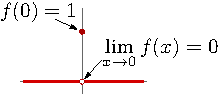
\includegraphics{03simple_discontinuity.pdf}}%
This function is not continuous at $x=0$ because $\lim_{x\to0} f(x) =
0$, while $f(0) = 1$: the limit for $x\to0$ exists, but it is
different from the function value at $x=0$.

This example is artificial, because we took a continuous function
($f(x) = 0$) and changed its definition at one point ($f(0) = 1$),
which then made the function discontinuous.  We get less artificial
examples by looking at functions that do not have limits.  If
$\lim_{x\to a} g(x)$ does not exist, then it certainly cannot be equal
to $g(a)$, and therefore any failed limit provides an example of a
discontinuous function.

For instance, the sign function $g(x) = \sign(x)$ from
\S~\ref{sec:sign-function-has-no-limit} is not continuous at $x=0$.
This kind of discontinuity is fairly common and has a name:
\marginpar{\input ../figures/221/03signOFx.tex\\
  \footnotesize\sffamily%
  $y=\sign (x)$: a function with a jump discontinuity.  Left and right
  limits at $x=0$ exist, but they are not the same}

\subsection{Definition}% of Jump discontinuity 
\itshape  A function $y=f(x)$ has a \emph{jump discontinuity} at $x=a$
if the left- and right-hand limits of $f(x)$  at $x=a$ both exist but are
different:
\[
\lim_{x\nearrow a} f(x) \neq \lim_{x\searrow a} f(x).
\]
\upshape

\subsection{Removable discontinuities} 
\label{sec:removable-discontinuities}
Consider the function from \S~\ref{sec:03xcos1overx}
\[
f(x) = x\cos\frac{\pi} {x}.
\]
It is defined for all $x$ except $x=0$, and therefore it is not continuous at
$x=0$, but for the silly reason that $f$ is not defined there: to decide if $f$
is continuous at $x=0$ we must compare $\lim_{x\to0} f(x)$ with $f(0)$,
but $f(0)$ isn't defined.  However, the limit
\[
\lim_{x\to 0} f(x) =\lim_{x\to 0} x \cos\frac{\pi} {x} = 0
\]
does exist (by the Sandwich theorem, see \S~\ref{sec:03xcos1overx}
again).
\marginpar{\input ../figures/221/03backwardCosSandwichSmall.tex}
Since $f(0)$ is not defined yet we can extend the
definition of $f$ to include $f(0) = 0$, i.e., we define
\[
g(x) =
\begin{cases}
  x\cos \pi/x & \text{ for }x\neq0\\
  0 & \text{ when }x=0 .
\end{cases}
\]
This new function $g(x)$ then is continuous everywhere, including at $x=0$.

This is an example of a more general situation in which the domain of
a function ``has a hole,'' meaning that the function is defined
everywhere in some interval $a-\delta <x < a+\delta$, except at $x=a$.
If the limit $\lim_{x\to a} f(x) = L$ exists, then you can extend the
definition of the function by declaring that $f(a) = L$.  The extended
function is then continuous at $x=a$.  The point $x=a$ is called a
\emph{removable discontinuity} of the function $f$.  In
\S~\ref{sec:another-example-of-removable-discontinuity} we'll see
another example of a function with a removable discontinuity whose
graph isn't as messy as the graph of $x\cos\pi/x$.


\section{Substitution in Limits} 
\label{sec:substitution-in-limits} Given
two functions $f$ and $g$, we can consider their composition $h(x) = f(g(x))$.
To compute the limit
\[
\lim_{x\to a} f\bigl(g(x)\bigr)
\]
we let $u=g(x)$, so that we want to know
\[
\lim_{x\to a}f(u) \text{ where }u=g(x).
\]
If we can find the limits
\[
L = \lim_{x\to a} g(x)\text{ and } \lim_{u\to L} f(u) = M,
\]
Then it seems reasonable that as $x$ approaches $a$, $u=g(x)$ will approach
$L$, and $f(g(x))$ approaches $M$.
This is in fact a theorem:
\subsection{Theorem} 
\label{thm:substitution}%
\itshape%
If $\lim_{x\to a}g(x) = L$, and if the function $f$ is continuous at $u=L$,
then
\[
\lim_{x\to a}f\bigl(g(x)\bigr) = \lim_{u\to L}f(u) = f(L).
\]\upshape

Another way to write this is
\[
\lim_{x\to a}f\bigl(g(x)\bigr) = f\bigl(\lim_{x\to a}g(x)\bigr).
\]
What this statement means is that we can freely move continuous functions outside of limits.
\subsection{Example: compute $\lim_{x\to3}\sqrt{x^3-3x^2+2}$} 
The given function is the composition of two functions, namely
\[
\sqrt{x^3-3x^2+2} = \sqrt u, \text{ with } u = x^3-3x^2+2,
\]
or, in function notation, we want to find $\lim_{x\to 3}h(x)$ where
\[
h(x) = f(g(x)), \text{ with } g(x) = x^3-3x^2+2\text{ and }f(x) = \sqrt{x}.
\]
Either way, we have
\[
\lim_{x\to 3}x^3-3x^2+2 = 2\quad\text{and}\quad \lim_{u\to 2}\sqrt u =
\sqrt 2.
\]
We can get the first limit from the limit properties $(P_1)$\ldots$(P_5)$.
The second limit says that taking the square root is a continuous function,
which it is. We have not proved this is true, but this particular limit is
the one from example \ref{ex:limit-of-sqrt-at-2}.  Putting these two limits
together, we conclude that the limit is $\sqrt2$.
% NOTE: if the subsection on continuous functions is written, rewrite this example!
We could more compactly write this whole argument as follows:
\[
\lim_{x\to3}\sqrt{x^3 - 3x^2 + 2} =\sqrt{\lim_{x\to 3}x^3 - 3x^2 + 2}
=\sqrt 2,
\]
with the remark that we need to know that $f(x)=\sqrt x$ is a continuous
function to justify the first step.

Another possible way of writing this is
\[
\lim_{x\to3}\sqrt{x^3 - 3x^2 + 2} =\lim_{u\to 2}\sqrt u =\sqrt2,
\]
where we would need to say that we have substituted $u=x^3-3x^2+2$.

\section{Problems} 
\problemfont 
\textit{Find the following limits:}\\
% !!! Issue: Some of these problems require "bad infinite limit reasoning" like in the subsection on that stuff.
\begin{multicols}{3}\setlength{\parindent}{0pt}

\problem $\DS \lim_{x\to -7}(2x+5) $ 

\problem $\DS \lim_{x\to 7-}(2x+5) $ 

\problem $\DS \lim_{x\to -\infty}(2x+5) $ 

\problem $\DS \lim_{x\to-4} (x+3)^{2006} $ 

\problem $\DS \lim_{x\to-4} (x+3)^{2007} $ 

\problem $\DS \lim_{x\to-\infty} (x+3)^{2007}$ 

\problem $\DS \lim_{t\to1}\frac{t^2+t-2}{t^2-1} $ 

\problem $\DS \lim_{t\nearrow1}\frac{t^2+t-2}{t^2-1} $ 

\problem $\DS \lim_{t\to-1}\frac{t^2+t-2}{t^2-1} $ 

\problem $\DS \lim_{x\to\infty}\frac{x^2+3}{x^2+4} $ 

\problem $\DS \lim_{x\to\infty}\frac{x^5+3}{x^2+4} $ 

\problem $\DS \lim_{x\to\infty}\frac{x^2+1}{x^5+2} $ 

\problem $\DS \lim_{x\to\infty} \frac{(2x+1)^4}{ (3x^2+1)^2} $ 

\problem $\DS \lim_{u\to\infty} \frac{(2u+1)^4}{ (3u^2+1)^2} $ 

\problem $\DS \lim_{t\to0} \frac{(2t+1)^4}{ (3t^2+1)^2}$ 
\end{multicols}
\problem What are the coordinates of the points labeled $A$, \ldots, $E$ in 
Figure~\ref{fig:03sinePiOverx} (the graph of $y=\sin\pi/x$).
\answer 
$A (\frac23,-1)$; $B (\frac25, 1)$; $C (\frac27,-1)$; $D(-1,0)$;
$E(-\frac25, -1)$.
\endanswer
% TO-DO: Combine all 10 or so of the true-false problems into one problem.
\problem If $\lim_{x\to a} f(x)$ exists then $f$ is continuous at $x=a$. 
\textit{True or false?}
\answer 
False!  The limit must not only exist \textit{but also be equal to
}$f(a)$!
\endanswer

\problem Give two examples of functions for which $\lim_{x\searrow 0} 
f(x)$ does not exist.
\answer 
There are of course many examples.  Here are two: $f(x) = 1/x$ and
$f(x) = \sin(\pi/x)$ (see \S\ref{sec:03backward-sine})
\endanswer

\problem \groupproblem If $\lim_{x\to 0}f(x)$ and $\lim_{x\to0}g(x)$ both do not 
exist, then $\lim_{x\to 0}\bigl(f(x) + g(x)\bigr)$ also does not exist.
\textit{True or false?}

\answer 
False!  Here's an example: $f(x) = \frac1x$ and $g(x) = x-\frac1x$.
Then $f$ and $g$ don't have limits at $x=0$, but $f(x) + g(x) = x$
\textit{does} have a limit as $x\to0$.
\endanswer

\problem \groupproblem If $\lim_{x\to 0}f(x)$ and $\lim_{x\to0}g(x)$ both do not 
exist, then $\lim_{x\to 0}(f(x)/g(x))$ also does not exist.  \textit{True or false?}

\answer 
False again, as shown by the example $f(x) = g(x) = \frac1x$.
\endanswer

\problem True or false: 

\subprob If $\lim_{x\to a} f(x)$ exists and $\lim_{x\to a} g(x)$ does
not exist, then $\lim_{x\to a} f(x) + g(x)$ could still exist.
\answer 
False, for the following reason:  $g(x)$ is the difference of $f(x)+g(x)$ and
$f(x)$.  If $\lim_{x\to a} f(x)$ exists and $\lim_{x\to a} f(x) + g(x)$ also exists, then
\begin{align*}
  \lim_{x\to a} g(x) &= \lim_{x\to a} \bigl\{f(x) + g(x) - f(x)\bigr\}\\
  &= \lim_{x\to a} \bigl\{f(x) + g(x)\bigr\} - \lim_{x\to a} f(x)
\end{align*}
also has to exist.
\endanswer

\subprob If $\lim_{x\to a} f(x)$ exists and $\lim_{x\to a} g(x)$ does
not exist, then $\lim_{x\to a} f(x) g(x)$ could still exist.
\answer 
True, as shown by the example $f(x) = x$, $g(x) = \frac{1}{x}$, and $a=0$.
For these two functions we have
\begin{gather*}
  \lim_{x\to 0} f(x) = 0 \text{ (i.e.\ exists) } \\
  \lim_{x\to 0} g(x) = \text{ does not exist } \\
  \lim_{x\to 0} f(x) g(x) = \lim_{x\to 0} x\times\frac1x = 1 \text{ (i.e.\
  exists) }
\end{gather*}
You can make up other examples, but to show that this statement is true you only
need one example.
\endanswer

\subprob If $\lim_{x\to a} f(x)$ exists and $\lim_{x\to a} g(x)$ does
not exist, then $\lim_{x\to a} f(x)/g(x)$ could still exist.
\answer 
True, as shown by the same example $f(x) = x$, $g(x) = \frac{1}{x}$, $a=0$.
This time we have
\begin{gather*}
  \lim_{x\to 0} f(x) = 0 \text{ (i.e.\ exists) } \\
  \lim_{x\to 0} g(x) = \text{ does not exist } \\
  \lim_{x\to 0} \frac{f(x)}{g(x)} = \lim_{x\to 0} \frac{x}{1/x} =\lim_{x\to0}
  x^2 = 0 \text{ (i.e.\ exists) }
\end{gather*}
You can make up other examples, but to show that this statement is true you only
need one example.
\endanswer

\subprob If $\lim_{x\to a} f(x)$ does not exist but $\lim_{x\to a} g(x)$ does
exist, then $\lim_{x\to a} f(x)/g(x)$ could still exist.
\answer 
False:  If $\lim_{x\to a} g(x)$ and $\lim_{x\to a} f(x)/g(x)$ both exist then
\begin{align*}
  \lim_{x\to a} f(x) &=
  \lim_{x\to a} g(x) \times \frac{f(x)}{g(x)} \\
  &\Bigl(\lim_{x\to a} g(x)\Bigr) \times \Bigl(\lim_{x\to a} \frac{f(x)}{g(x)}\Bigr) \\
\end{align*}
and therefore $\lim_{x\to a} f(x)$ would also have to exist.
\endanswer

\problem \label{ex:limx-dne} \groupproblem In the text we proved that 
$\lim_{x\to\infty} \frac1x=0$.  Show that this implies that
$\lim_{x\to\infty}x$ does not exist.  Hint: Suppose $\lim_{x\to\infty}x =
L$ for some number $L$.  Apply the limit properties to
$\lim_{x\to\infty}x\cdot (\frac1x)$.
\bigskip

\begin{multicols}{2}\setlength{\parindent}{0pt}
\problem Evaluate $\DS \lim_{x\to 9}\frac{\sqrt x- 3}{x-9}$.  Hint: Multiply top 
and bottom by $\sqrt x+3$.

\problem Evaluate $\DS \lim_{x\to 2}\frac{\frac1x-\frac12}{x-2}$. 

\problem  Evaluate $\DS \lim_{x\to 2}\frac{\frac1{\sqrt{x}}-\frac1{\sqrt2}}{x-2}$. 

\problem  A function $f$ is defined by 
\[
f(x)= \begin{cases}
  x^3 & \text{ for } x<-1\\
  ax+b & \text{ for } -1 \leq x <1\\
  x^2 +2 & \text{ for } x \geq 1.
\end{cases}
\]
where $a$ and $b$ are constants.  The function $f$ is continuous. What
are $a$ and $b$?

\problem Find a constant $k$ such that the function 
\[
f(x)= \begin{cases}
  3x+2 & \text{for }   x <2\\
  x^2 +k & \text{for }x \geq 2.
\end{cases}
\]
is continuous.  Hint: Compute the one-sided limits.

\problem Find all possible pairs of constants $a$ and $c$ such that the function 
\[
f(x)=
\begin{cases}
  x^3+c & \text{for } x<0\\
  ax+c^2 & \text{for } 0 \leq x <1\\
  \arctan x & \text{for }x \geq 1.
\end{cases}
\]
is continuous for all $x$. (There is more than one possibility.)
\end{multicols}


%%%%%%%%%%%%%%%%%%%%%%%%%%%%%%%
\noproblemfont
\section{Two Limits in Trigonometry} 
\label{sec:trigLimit}

In this section we derive a few limits involving the trigonometric
functions.  You can think of them as saying that for small angles $\theta$
one has
\begin{equation}
  \sin\theta \approx \theta\quad\text{and}\quad \cos\theta\approx 1-\tfrac12
  \theta^2.
  \label{eq:03sine-theta-is-roughly-theta}
\end{equation}
We will use these limits when we compute the derivatives of Sine, Cosine
and Tangent.

\subsection*{Theorem}% 
\begin{equation}
  \lim_{\theta\to 0}\frac{\sin\theta}{\theta} = 1 .
  \label{eq:03trig-limit}
\end{equation}

\begin{figure}[t]
  \framebox{
    \parbox[b]{0.4\textwidth}{ 
%    \begin{picture} (180.000000,117.306957)(0,0)
    \begin{picture} (0,0)(0,50)
    \put(0.0, 0.0){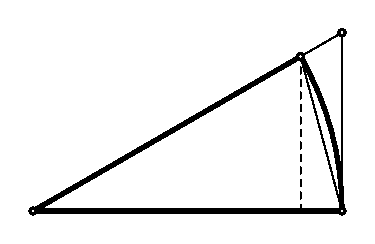
\includegraphics{03dsin.pdf}}
        \put( 15.83,   3.83){\sffamily\itshape $O$}
    \put(164.17,   3.83){\sffamily\itshape $A$}
    \put(161.17, 107.47){\sffamily\itshape $B$}
    \put(141.29,  96.00){\sffamily\itshape $C$}
    \put(157.31,  68.99){\sffamily\itshape $\theta$}
    \put(168.17,  53.65){\sffamily\itshape \rotatebox{90}{$\tan\theta$}}
    \put(134.29,  47.92){\sffamily\itshape \rotatebox{90}{$\sin\theta$}}
\end{picture}
}
  \hspace{0.15\textwidth}
  \begin{minipage}{0.4\textwidth}
    \setlength{\parskip}{1ex plus 1ex}\footnotesize \sffamily
    \raggedright
    \rule{0pt}{16pt}

    The circular wedge $OAC$ contains the triangle $OAC$ and is contained
    in the right triangle $OAB$.

    The area of triangle $OAC$ is $\frac12\sin\theta$.

    The area of circular wedge $OAC$ is $\frac12\theta$.

    The area of right triangle $OAB$ is $\frac12\tan\theta$.

    Hence one has \( \sin\theta < \theta < \tan\theta \) for all angles
    $0<\theta<\pi/2$.  \vspace{10ex}\null
  \end{minipage}
  }
  \caption{Proving $\lim_{\theta\to 0} \dfrac{\sin \theta}{\theta}
    = 1$ by comparing the areas of two triangles and a circular wedge. }
  \label{fig:sintheta-almost-theta}
\end{figure}

\begin{proof}
  The proof requires a few sandwiches and some geometry.  We begin by
  only considering positive angles, and in fact we will only consider
  angles $0<\theta<\pi/2$.

  Look at Figure~\ref{fig:sintheta-almost-theta}.   Since the wedge
  $OAC$ contains the triangle $OAC$ its area must be larger.  The area
  of the wedge is $\frac12\theta$ and the area of the triangle is
  $\frac12\sin \theta$, so we find that
  \begin{equation}\label{eq:03SineBelowTheta}
    0<\sin \theta <\theta \text{ for } 0<\theta<\frac\pi2.
  \end{equation}
  The Sandwich Theorem implies that
  \begin{equation}\label{eq:03limSineisZero}
    \lim_{\theta\searrow 0}\sin\theta = 0.
  \end{equation}
  Moreover, we also have
  \begin{equation}\label{eq:03limCosisOne}
    \lim_{\theta\searrow0}\cos\theta =
    \lim_{\theta\searrow0}\sqrt{1-\sin^2\theta} = 1.
  \end{equation}

  Next we compare the areas of the wedge $OAC$ and the larger triangle
  $OAB$.  Since $OAB$ has area $\frac12\tan \theta$ we find that
  \[
  \theta<\tan\theta
  \]
  for $0<\theta<\frac\pi2$.  Since $\tan\theta =
  \frac{\sin\theta}{\cos\theta}$ we can multiply with $\cos\theta$ and
  divide by $\theta$ to get
  \[
  \cos\theta < \frac{\sin\theta}{\theta} \text{ for }0<\theta<\frac\pi2
  \]
  If we go back to \eqref{eq:03SineBelowTheta} and divide by $\theta$, then we
  get
  \[
  \cos\theta < \frac{\sin\theta}{\theta} < 1
  \]
  The Sandwich Theorem can be used once again, and now it gives
  \[
  \lim_{\theta\searrow0} \frac{\sin\theta}\theta = 1.
  \]
  This is a one-sided limit.  To get the limit in which $\theta\nearrow 0$,
  you use that $\sin\theta$ is an odd function.
\end{proof}

\subsection{The Cosine counterpart of \eqref{eq:03trig-limit}} 
We will show that
\begin{equation}
  \lim_{\theta\to 0}\frac{1-\cos\theta}{\theta^2} = \frac12.
  \label{eq:03CosLimit}
\end{equation}

This follows from $\sin^2\theta+\cos^2\theta=1$.  Namely,
\begin{align*}
  \frac{1-\cos\theta}{\theta^2}
  &= \frac1{1+\cos\theta}\,\frac{1-\cos^2\theta}{\theta^2} \\
  &= \frac1{1+\cos\theta}\,\frac{\sin^2\theta}{\theta^2} \\
  &= \frac1{1+\cos\theta}\left( \frac{\sin\theta}{\theta} \right)^2.
\end{align*}
We have just shown that $\cos\theta\to1$ and $\frac{\sin\theta}\theta \to
1$ as $\theta\to0$, so \eqref{eq:03CosLimit} follows.

This limit claims that for small values of $\theta$ one has
\[
\frac{1-\cos\theta}{\theta^2} \approx \frac{1}{2},
\]
and hence
\[
\cos \theta \approx 1 - \frac{1}{2}\theta^2.
\]


\subsection{The Sine and Cosine of a small angle} 
As promised in  \eqref{eq:03sine-theta-is-roughly-theta}, you can use
the limits in this section to approximate $\sin\theta$ when $\theta$
is small.  Namely, since $\lim_{\theta\to0}\frac{\sin\theta}{\theta} = 1$ it is
reasonable to assume that for small angles $\theta$ one has
$\frac{\sin\theta}{\theta}\approx 1$, or, $\sin\theta \approx \theta$.
Similarly, \eqref{eq:03CosLimit} implies that for small angles
$\theta$ one has $\cos\theta \approx 1 - \frac12\theta^2$.

For instance, to get a quick estimate of $\sin(0.1)$ and $\cos(0.1)$
(where, as always, $0.1$ is measured in radians)
we use \eqref{eq:03sine-theta-is-roughly-theta} and get
\[
\sin 0.1 \approx 0.1, \qquad
\cos 0.1 \approx 1-\tfrac12(0.1)^2 = 0.995.
\]
The formula \eqref{eq:03sine-theta-is-roughly-theta} does not say how
accurate these approximations are.  To see how good the approximations
are you could compare with the actual values of $\sin 0.1$ and $\cos
0.1$.  These are, rounded to six decimals,
\[
\sin 0.1 \approx 0.099\,833,\qquad
\cos 0.1 \approx 0.995\,004.
\]

\subsection{Another example of a removable discontinuity} 
\label{sec:another-example-of-removable-discontinuity}
Since $(\sin x) /x\to1$ as $x\to0$, the function $f(x) = \frac{\sin x}
{x}$ has a removable discontinuity at $x=0$ (see
\S~\ref{sec:removable-discontinuities}.)

\centerline{\input ../figures/221/03sinx-over-x.tex}

\noindent%
The function
\[
f(x) \stackrel{\rm def}=
\begin{cases}
  (\sin x)/x & \text{for }x\neq0,\\
  1 & \text{when }x=0
\end{cases}
\]
is continuous at $x=0$.

\section{Problems} 
\problemfont 
\noindent\itshape
For each of the following limits, either evaluate them \emph{or} show that they
do not exist.  Distinguish between limits which are infinite and limits which do
not exist.\upshape

\begin{multicols}{3}\setlength{\parindent}{0pt}
\problem $\DS \lim_{\theta\to0} \frac{\tan \theta}{\theta}$ 

(Hint: $\tan\theta = \frac{\sin\theta}{\cos \theta}$).
\answer 
the limit is 1.
\endanswer

\problem $\DS \lim_{\theta\to0} \frac{\theta}{\sin \theta}$ 

\answer 
The limit is 1.
Use :
$\frac{\theta}{\sin\theta} = \frac{1}{\frac{\sin\theta}{\theta}}$.
\endanswer

\problem $\DS \lim_{\alpha\to0}\frac{\sin 2\alpha}{\alpha}$ 

(Hint: a substitution)

\problem $\DS \lim_{\alpha\to0}\frac{\sin 2\alpha}{\sin\alpha}$ 

(two ways: with and without the double angle formula!)
\answer 
$\sin 2\alpha = 2\sin\alpha\cos\alpha$ so the limit is
$\lim_{\alpha\to0} \frac{2\sin\alpha\cos\alpha}{\sin\alpha} =
\lim_{\alpha\to0} 2\cos\alpha = 2$.

Other approach: $\DS\frac{\sin2\alpha}{\sin\alpha} =
\frac{\frac{\sin2\alpha}{2\alpha}}{\frac{\sin\alpha}{\alpha}}\cdot
\frac{2\alpha}{\alpha}$. Take the limit and you get 2.
\endanswer

\problem $\DS \lim_{x\to0}\frac{\sin 3x}{2x}$. 

\answer 
$\frac{3}{2}$.
\endanswer



\problem $\DS \lim_{\alpha\to0}\frac{\tan 4\alpha}{\sin 2\alpha}$. 

\answer 
$\frac{\tan 4\alpha}{\sin 2\alpha}
= \frac{\tan 4\alpha}{4\alpha}\cdot
\frac{4\alpha}{2\alpha}\cdot \frac{2\alpha}{\sin2\alpha}$.

Take the limit and you get $\ldots = 1\cdot1\cdot2 = 2$.
\endanswer

\problem $\DS \lim_{x\to 0} \frac{1-\cos x}{ x \sin x}.$ 

\answer 
Hint: multiply top and bottom with \(1+\cos x\).
\endanswer

\problem $\DS\lim_{\theta\to\pi/2}\frac{1-\sin\theta}{\theta-\pi/2}$ 

\answer 
Hint: substitute $\theta = \frac{\pi}{2} - \varphi$, and let $\varphi\to 0$.  Answer: $0$.
\endanswer

\problem $\DS \lim_{x\to0}\frac{\sin^2 x}{1-\cos x}$. 
\answer 
Multiply top and bottom with $1+\cos x$.  The answer is $2$.
\endanswer
\problem $\DS \lim_{x\to0}\frac{\sin(x^2)}{x^2}.$ 
\answer 
Substitute $x^2 = u$ and let $u\to 0$.  Answer: $1$.
\endanswer

\problem $\DS \lim_{x\to 0} \frac{x(1-\cos x)}{ \tan^3 x}.$ 
\answer 
Multiply and divide by $1+\cos x$.  Write $\tan x$ as $\frac{\sin x}{\cos x}$.
Answer is $\frac12$.
\endanswer
\problem $\DS \lim_{x\to 0} \frac{\sin(x^2)}{ 1-\cos x}. $ 
\answer 
$\DS \frac{\sin(x^2)}{ 1-\cos x} = \frac{\sin (x^2)}{x^2} \frac{x^2}{1-\cos x}$.
The answer is $2$.
\endanswer
\problem \(\DS\lim_{x\to\pi/2}\frac{x-\tfrac\pi2}{\cos x}\). 
\answer 
Substitute \(\theta = x-\pi/2\) and remember that \(\cos x = \cos(\theta+\frac\pi2) = -\sin\theta\).  You get
\[
\lim_{x\to\pi/2}\frac{x-\tfrac\pi2}{\cos x} =\lim_{\theta\to0}
\frac{\theta}{-\sin\theta} = -1.
\]
\endanswer

\problem \(\DS\lim_{x\to\pi/2}(x-\tfrac\pi2)\tan x\). 

\answer 
Similar to the previous problem, once you use \(\tan x = \frac{\sin
  x}{\cos x}\). The answer is again \(-1\).
\endanswer

\problem $\DS \lim_{x\to 0}\frac{\cos x}{x^2+9}.$ 
\answer 
$1/9$
\endanswer

\problem $\DS \lim_{x\to \pi}\frac{\sin x}{x-\pi}.$ 

\answer 
Substitute \(\theta = x-\pi\).  Then \(\lim_{x\to\pi}\theta=0\), so
\[
\lim_{x\to \pi}\frac{\sin x}{x-\pi} = \lim_{\theta\to0}
\frac{\sin(\pi+\theta)}{\theta} = -\lim_{\theta\to0}
\frac{\sin\theta}{\theta} = -1.
\]
Here you have to remember from trigonometry that \(\sin(\pi+\theta)
= -\sin\theta\).
\endanswer

\problem $\DS \lim_{x\rightarrow 0}\frac{\sin x}{x+\sin x}.$ 
\answer 
Divide top and bottom by $x$.  The answer is $1/2$.
\endanswer

\problem \carefulnow $\DS A = \lim_{x\to\infty} \frac{\sin x}{x}$. 

\answer 
Note that the limit is for \(x\to\infty\)!  As \(x\) goes to
infinity \(\sin x\) oscillates up and down between \(-1\) and
\(+1\).  Dividing by \(x\) then gives you a quantity which goes to
zero.  To give a good proof you use the Sandwich Theorem like this:
\smallskip

Since \(-1\le \sin x\le 1\) for all \(x\) you have
\[
\frac{-1}{x} \le \frac{\sin x}{x} \le \frac{1}{x}.
\]
Since both \(-1/x\) and \(1/x\) go to zero as \(x\to\infty\) the
function in the middle must also go to zero.  Hence
\[
\lim_{x\to\infty} \frac{\sin x}{x} = 0.
\]
\endanswer

\problem $\DS B = \lim_{x\to\infty} \frac{\cos x}{x}$. 

\answer 
zero again.
\endanswer

\problem \carefulnow $\DS\lim_{x\to\infty} \frac{\tan x}{x}$ 

\problem $\DS\lim_{x\to\infty} \frac{\sin 2x}{x}$ 

\problem $\DS \lim_{x\to\infty} \frac{\sin 2x}{1+x^2}$ 

\problem $\DS \lim_{x\to\infty} \frac{x}{\cos x + x^2}$ 
\answer 
This is not a rational function, but you can use the same trick:  factor out the
highest power of $x$ from numerator and denominator.  You get
\[
 \frac{x}{\cos x + x^2}
 = \frac{x}{x^2} \frac{1}{\frac{\cos x}{x^2} + 1}.
\]
Using the Sandwich Theorem as in the previous problems you get
$\lim_{x\to\infty} \frac{\cos x}{x^2} = 0$.  With the limit properties you then
get
\begin{align*}
  \lim_{x\to\infty}\frac{x}{\cos x + x^2}
 &= \lim_{x\to\infty}\frac{x}{x^2} \frac{1}{\frac{\cos x}{x^2} + 1}\\
 &= 0\times \frac{1}{0+1} \\
 &= 0.
\end{align*}

\endanswer
\problem $\DS \lim_{x\to\infty} \frac{2x^3+3x^2\cos x }{ (x+2)^3}$ 
\answer 
$2$.
\endanswer

\end{multicols}

\begin{multicols}{2}\setlength{\parindent}{0pt}
\problem Since both $\lim_{\theta\to0}\frac{\sin\theta}{\theta} = 1$ and 
$\lim_{\theta\to0}\frac{\tan\theta}{\theta} = 1$, you would think that
for small angles $\theta$
\[
\sin\theta \approx \theta \approx \tan\theta.
\]
In other words the sine and tangent of small angles are almost the
same.  This problem goes into the question of how small the
difference really is.

\subprob Compute $\DS \lim_{\theta\to0}\frac{\tan\theta -
\sin\theta}{\theta^3}$.  

(Hint:  use $\tan\theta = \sin\theta/\cos\theta$.)
\answer 
$\DS \lim_{\theta\to0}\frac{\tan\theta - \sin\theta}{\theta^3} =
\frac{1}{2}$
\endanswer

\subprob  Use your answer from part (a) to estimate the difference
between $\tan 0.1$ and $\sin 0.1$.
\answer 
$\tan0.1 - \sin 0.1 \approx \frac{1}{2}(0.1)^{3} = 0.0005$, which is
really a lot smaller than $0.1$.
\endanswer

\problem Suppose you are lost on an island and you have no calculator. 
Approximate the following quantities as best as you can:

\subprob $\sin{0.2}$
\hfill
\subprob $\cos{0.2}$
\hfill
\subprob $\tan{0.2}$

\subprob $\sin\bigl(\frac\pi2 - {0.2}\bigr)$
\hfill
\subprob $\cos\bigl(\frac\pi2 + {0.2}\bigr)$
\hfill
\subprob $\tan\bigl(\frac\pi2 - {0.2}\bigr)$
\setcounter{SUBPROB}{0}
\answer 
$\sin0.2 \approx 0.2$,

$\cos{0.2} \approx 1-\frac12(0.2)^2 = 0.98$,

$\tan{0.2} = (\sin{0.2})/(\cos{0.2}) \approx 0.2$.

$\sin \bigl(\pi/2 - 0.2\bigr) = \cos 0.2 \approx 0.98$.

$\cos \bigl(\pi/2 + 0.2\bigr) = -\sin 0.2 \approx -0.2$.

$\tan \bigl(\pi/2 - 0.2\bigr) = \dfrac1{\tan 0.2} \approx \dfrac1{0.2} = 50$.

\endanswer
\problem You are still on the island, and you still have no 
calculator.  Approximate the following quantities as best as you can:

\subprob $\sin10^\circ$
\hfill
\subprob $\cos10^\circ$
\hfill
\subprob $\tan10^\circ$


\subprob $\sin100^\circ$
\hfill
\subprob $\cos10^\circ$
\hfill
\subprob $\tan80^\circ$

\carefulnow\ \  Note that here the angles are specified in degrees rather
than radians.

\setcounter{SUBPROB}{0}
\answer 
Same approach as before, but in this problem you first have to convert
$10^\circ$ to radians:
\[
10^\circ = \frac{10}{360}\times2\pi \textrm{radians} = \frac{\pi}{18}.
\]
You get
\[
\sin 10^\circ \approx \frac{\pi}{18},
\]
\[
\cos 10^\circ \approx 1 - \frac{\pi^2}{2\times18^2}.
\]
You don't have a calculator, so, had this been 1965, you would have
enthusiastically computed these numbers by hand (to two decimals).

For a really rough estimate assume $\pi\approx3$, to get
\[
10^\circ \approx \frac{3}{18} = \frac{1}{6} \approx 0.17,
\]
\[
\tan 10^\circ \approx \sin 10^\circ \approx \frac{3}{18} = \frac{1}{6} \approx
0.17,
\]
\begin{align*}
  \cos 10^\circ &\approx 1 - \frac{1}{2} \bigl(\frac{1}{6}\bigr)^2\\
  &= 1- \frac{1}{72}\\
  &\approx 1-0.014 = 0.986
\end{align*}
To find the other expressions, use $\sin(\frac\pi2+\theta) =
\cos\theta$ and $100^\circ = 90^\circ + 10 ^\circ$.

$\sin 100^\circ = \cos10^\circ \approx -0.986 $

$\cos 190^\circ = -\cos 10^\circ \approx -0.986$

$\tan80^\circ = \bigl(\tan 10^\circ\bigr)^{-1} \approx 6$ .
\endanswer

\problem \subprob Simplicio says that while a \textit{million} is clearly a lot, 
\textit{two} is not a large number.  After reading
\eqref{eq:03sine-theta-is-roughly-theta} he then concludes that
\[
\sin(2) \approx 2.
\]
Comment on his conclusion, and explain the meaning of ``small'' in
the sentence ``\textit{if $\theta$ is small then $\sin\theta \approx
\theta$.}''

\subprob The next day Simplicio makes an accurate drawing of a three
degree angle by dividing a right angle ($90^\circ$) into $30$ equal
angles.  The drawing convinces him that three degrees is a very small
angle indeed, and so he concludes that
\[
\sin 3^\circ \approx 3.
\]
Again, comment on Simplicio's reasoning.

\problem Is there a constant $k$ such that the function 
\[
f(x)= \begin{cases}
  \sin(1/x) &\text{for }x\ne 0\\
  k & \text{for } x=0.
\end{cases}
\]
is continuous?  If so, find it; if not, say why no such $k$ exists.
\answer 
No.  As \(x\to0\) the quantity \(\sin \frac{1}{x}\) oscillates
between \(-1\) and \(+1\) and does not converge to any particular
value.  Therefore, no matter how you choose \(k\), it will never be
true that \(\lim_{x\to 0} \sin \frac1x = k\), because the limit
doesn't exist.
\endanswer

\problem Find a constant \(A\) so that the function 
\[
f(x) =
\begin{cases}
  \dfrac{\sin x}{2x} &\hbox{for $x\ne0$} \\
  A & \hbox{when \(x=0\)}
\end{cases}
\]
  is continuous everywhere.
\answer 
The function \(f(x) = (\sin x)/x\) is continuous at all \(x\ne 0\),
so we only have to check that \(\lim_{x\to0} f(x) = f(0)\), i.e.\
\(\lim_{x\to0}\frac{\sin x}{2x} = A\).  This only happens if you
choose \(A=\frac12\).
\endanswer

\problem Compute $\lim_{x\toi}x\sin\frac \pi x$ and $\lim_{x\toi}x 
\tan\frac\pi x$. (Hint: substitute something).


\end{multicols}
\noproblemfont


\section{Asymptotes} 
\label{sec:asymptotes}
Asymptotes can be vaguely defined by saying that a line is an
asymptote of the graph of a function $y=f(x)$ if the graph ``approaches the line
as $x$ approaches infinity.'' For a more precise definition we distinguish
between three cases, depending on the line.

\subsection{Vertical Asymptotes} 
If $y=f(x)$ is a function for which either
\[
\lim_{x\searrow a} f(x) = \infty,
\text{ or }
\lim_{x\searrow a} f(x) = -\infty,
\text{ or }
\lim_{x\nearrow a} f(x) = \infty,
\text{ or }
\lim_{x\nearrow a} f(x) = -\infty
\]
holds, then the line $x=a$ is a \emph{vertical asymptote} of the function $y=f(x)$.

\subsection{Horizontal Asymptotes} 
If $y=f(x)$ is a function for which
\[
\lim_{x\to \infty} f(x) = a \text{ or }
\lim_{x\to-\infty} f(x) = a,
\]then the line $y=a$ is a \emph{horizontal asymptote} of the function
$y=f(x)$.

\subsection{Slanted Asymptotes} 
\label{sec:03slanted-asymptotes}
If $y=f(x)$ is a function for which
\[
\lim_{x\to\infty} \left[ f(x) - \bigl(mx+n\bigr)\right] =0,\text{ or }
\lim_{x\to-\infty} \left[ f(x) - \bigl(mx+n\bigr)\right] =0,
\]
then the line $y=mx+n$ is a \emph{slanted asymptote} for the function
$y=f(x)$.
In this case we say that \emph{the function $f(x)$ is asymptotic to
$mx+n$ as $x\to\infty$} (or $x\to-\infty$, depending on the case).

Slanted asymptotes are the hardest to find, but the following
observations can be helpful.  

\subsection{Asymptotic slope and intercept} 
If $y=mx+n$ is a slanted asymptote of $y=f(x)$ then
\begin{equation}
  m = \lim_{x\to\infty} \frac{f(x)}{x}, \qquad
  n = \lim_{x\to\infty} f(x) - mx.
  \label{eq:03asymptotic-slope-intercept}
\end{equation}
You should be able to prove this yourself. See
problem~\ref{ex:prove-asymptotic-slope-intercept}.
% !!! TO-DO: and conversely, if these two limits exist then the function has y=mx+n as a slant asymptote.

\begin{figure}[bt]
  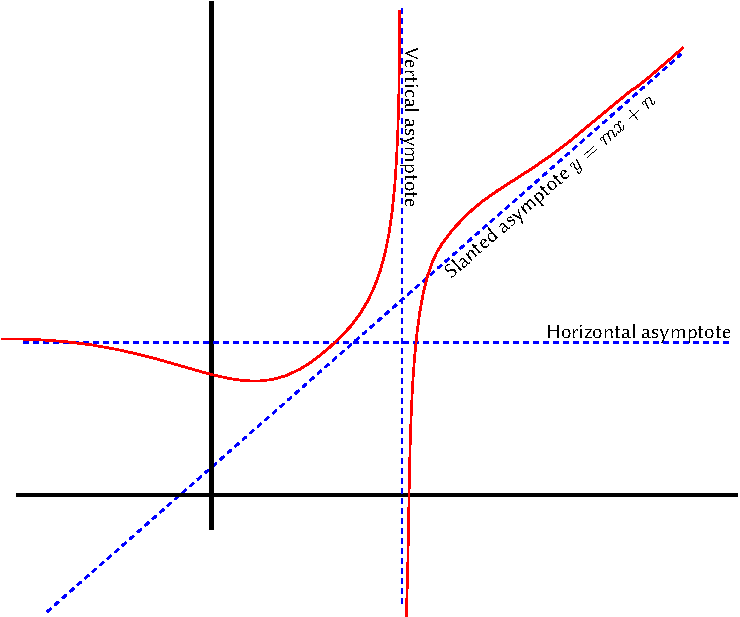
\includegraphics[width=0.6\textwidth]{03asymptotes.pdf}
  \caption{A function with all three kinds of asymptote. }
  \label{fig:03asymptotes}
\end{figure}

\subsection{Example} 
The function
\[
f(x) = \dfrac x{1-x}
\]
has both a horizontal and a vertical asymptote.  To find the
vertical asymptote we look for values of $x$ where the function
``may become infinite.'' The function is well defined everywhere
except when the denominator $1-x$ vanishes.  This happens when $x=1$.
To verify that $x=1$ is a vertical asymptote we compute the limit
\[
\lim_{x\searrow1} f(x) = -\infty \text { and }
\lim_{x\nearrow1} f(x) = +\infty.
\]
Either of these two limits shows that the line $x=1$ is a vertical
asymptote for $y= x/(1-x)$.

To find the horizontal asymptotes we compute
\[
\lim_{x\to\infty} f(x) = -1
\text{ and }
\lim_{x\to-\infty} f(x) = -1.
\]
Again, either of these limits implies that the line $y=-1$ is a
horizontal asymptote for $y=x/(1-x)$.

\subsection{Example} 
Find the asymptotes of the function
\[
f(x) = \sqrt{x^2+1}.
\]
The function is well defined and continuous at all $x$.  This means
that $\lim_{x\to a} f(x)$ is always finite (it's $f(a)$) and therefore
this function has no vertical asymptotes.

Both limits $\lim_{x\to\pm\infty} f(x)$ are infinite so the function
also has no horizontal asymptotes.  

To find possible slanted asymptotes we first see what the slope of
such an asymptote would be:
\[
m
= \lim_{x\to\infty}\frac{f(x)}{x}
= \lim_{x\to\infty}\frac{\sqrt{x^2+1}}{x}
= \lim_{x\to\infty}\sqrt{1+\frac{1}{x^2}} = 1.
\]
This does not yet prove that there is a slanted asymptote; to prove
that one exists we must also find the intercept of the asymptote.
This intercept is given by
\[
n = \lim_{x\to\infty} f(x) - mx
=\lim_{x\to\infty} \sqrt{x^2+1} - x
  = \lim_{x\to\infty} \frac{1}{\sqrt{x^2+1} + x}
  = \lim_{x\to\infty} \frac{1/x}{\sqrt{1+1/x^2} + 1}
  = \dfrac{0}{2}.
\]
This last limit implies that
\[
\lim_{x\to\infty} f(x) - x = 0
\]
and therefore $y=x$ is the slanted asymptote of the function.

\section{Problems} 
\problemfont 
\begin{multicols}{2}
\problem Find the asymptotes (horizontal, vertical and slanted) of the 
following functions:

\subprob $\DS f(x) = \frac{x}{x^2+1}$

\subprob $\DS f(x) = \frac{x}{x^2-4}$

\subprob $\DS f(x) = \frac{5x^2}{x^2-2}$

\subprob $\DS f(x) = \frac{x}{x^2-4}$

\subprob $\DS f(x) = \frac{x}{x-4}$

\subprob $\DS f(x) = \frac{x^3}{x^2+4}$

\problem Which of the following functions have asymptotes? 

\subprob \(\DS f(x) = \sqrt{x} \)
\answer 
No vertical asymptote.  
No horizontal asymptote.  
If there were a slanted asymptote then $m =
\lim_{x\to\infty}\frac{\sqrt{x}}{x} = 0$. But $n = \lim_{x\to\infty}
f(x) - mx = \lim_{x\to\infty}\sqrt{x}$ does not exist.
\endanswer

\subprob \(\DS f(x) = \sqrt{x} - \sqrt{x-1}\)

\subprob \(\DS f(x) = x+ \cos x \)

\subprob \(\DS f(x) = x\sin x \)

\subprob \(\DS f(x) = \dfrac{\sin x}{x} \)

\subprob $\DS f(x) = \sqrt{x^2+x}$

\subprob $\DS f(x) = \frac{x}{\sqrt{x^2+1}}$

\problem Find all asymptotes for the graphs of the following functions: 

\subprob $\DS f(x) = \frac{\sin x}{x^2+4}$

\subprob $\DS f(x) = \frac{\sin x}{x-\pi}$

\subprob $\DS f(x) = \frac{\sin x}{x-1}$

\subprob $\DS f(x) = \tan x$

\subprob $\DS f(x) = \sec \frac x2$

\subprob $\DS f(x) = \arctan x$

\subprob $\DS f(x) = \arctan (x/\pi)$

\subprob $\DS f(x) = \dfrac{\arctan x}{x}$

\subprob $\DS f(x) = \tan \pi x$

\subprob $\DS f(x) = \sec (x^2)$

\problem Give an example of a function $y=f(x)$ that is defined for 
all $x>0$, whose graph has no slanted asymptote, but which still satisfies
\[
\lim_{x\to\infty} \frac{f(x)}{x} = 1.
\]
\problem \textbf{Do a proof!}  Derive the formulas 
\eqref{eq:03asymptotic-slope-intercept}
\label{ex:prove-asymptotic-slope-intercept}
from the definition of slanted asymptote in
\S\ref{sec:03slanted-asymptotes}.

\textit{About finding proofs}:  you can use all the material in this chapter of
the text.  Proofs usually don't ``just come to you.'' Instead they tend to
require some puzzling and most often our first few written attempts at the proof
belong in the trash.  The proof we keep for posterity should be a short and
polished write-up of the argument we find.
\answer 
We are given that
\[
\lim_{x\to\infty} f(x) - mx-n = 0.
\]
Adding $n$ to both sides gives us
\[
\lim_{x\to\infty} f(x) -mx = n,
\]
which is the formula for $n$ we had to prove.

To get the formula for $m$ we multiply with
\[
\lim_{x\to\infty} 1/x =
0
\]
and use the limit properties:
\begin{multline*}
  \lim_{x\to\infty} \frac{f(x)-mx-n}{x} = \\
  \bigl(\lim_{x\to\infty} f(x)-mx-n\bigr)\times
  \bigl(\lim_{x\to\infty}\frac{1}{x}\bigr)=\\
  0\times0 = 0.
\end{multline*}
Work out the left hand side:
\[
0 = \lim_{x\to\infty} \frac{f(x)}{x} - m - \frac{n}{x}.
\]
This implies
\[
0 = \lim_{x\to\infty} \frac{f(x)}{x} - m
\]
and thus
\[
\lim_{x\to\infty} \frac{f(x)}{x} = m.
\]

\endanswer
\problem Suppose the function $y=f(x)$ has exactly one vertical 
asymptote, which happens to be located at $x=1$.  
Which of the following functions have vertical asymptotes, and where
are they located?

\subprob  $g(x) = f(2x)$

\subprob  $h(x) = xf(x)$

\subprob  $h(x) = (x-1)f(x)$

\subprob  $k(x) = f(x)+\sin x$

\end{multicols}
\noproblemfont

%%% Local Variables:
%%% mode: latex
%%% TeX-master: "free221"
%%% End:
